\documentclass[11pt]{article}
\usepackage[utf8]{inputenc}
\usepackage[T1]{fontenc}
\usepackage{textcomp}
\usepackage[a4paper,margin=2.1cm]{geometry}
\usepackage{amsmath,amssymb}
\usepackage{graphicx}
\usepackage{tikz}
\usetikzlibrary{positioning,arrows.meta,calc}
\usepackage{xcolor}
\usepackage{mdframed}
\usepackage[colorlinks=true,linkcolor=blue!60!black]{hyperref}
\setlength{\parindent}{0pt}
\setlength{\parskip}{6pt}

\newcommand{\question}[1]{\par\medskip\noindent\textbf{#1}\par}
\newmdenv[linecolor=green!45!black,linewidth=0.8pt,backgroundcolor=green!4,
  innertopmargin=4pt,innerbottommargin=4pt,skipabove=6pt,skipbelow=6pt]{answerbox}

\title{\textbf{Laws of Surds}\\[0.3em]\large Worked Solutions with TikZ Diagrams}
\author{Wisest Maths --- Year 1 A-Level, Algebra (ref \texttt{a5})}
\date{}

\begin{document}
\maketitle
\noindent This document contains all 40 \emph{Laws of Surds} questions, each with a fully worked
solution and a TikZ diagram matched to the task:
\begin{itemize}\setlength{\itemsep}{1pt}
  \item \textbf{Factor trees} for simplifying $\sqrt{n}$ (split off the largest perfect square);
  \item \textbf{Surd-law cards} for multiplying, squaring and fraction surds;
  \item \textbf{Area-model (box) grids} for expanding brackets, difference of two squares and perfect squares;
  \item \textbf{Solution-flow} diagrams for adding/subtracting surds and fraction products;
  \item a \textbf{right-triangle} diagram for the Pythagoras problem.
\end{itemize}
\tableofcontents
\bigskip
\hrule

\section*{Laws of Surds 01\quad\small\texttt{(a5-001)}}
\addcontentsline{toc}{section}{Laws of Surds 01 (a5-001)}
\textit{Difficulty: Foundation \quad\textbar\quad Marks: 1}

\question{Simplify: \( \sqrt{12} \)}

\textbf{Worked solution.}

\textit{Step 1: Find the largest square number that is a factor of 12.}
\[\begin{gathered}
\sqrt{12} = \sqrt{4 \times 3}
\end{gathered}\]
4 is the largest square number that divides into 12.

\textit{Step 2: Split using the rule \( \sqrt{ab} = \sqrt{a} \times \sqrt{b} \) and simplify.}
\[\begin{gathered}
\sqrt{4} \times \sqrt{3} = 2\sqrt{3}
\end{gathered}\]
\( \sqrt{4} = 2 \), so the surd simplifies to \( 2\sqrt{3} \).

\begin{answerbox}
\textbf{Final answer:}\quad \(\displaystyle 2\sqrt{3}\)
\end{answerbox}
\textbf{Diagram.}

\begin{center}
\resizebox{\ifdim\width>\linewidth \linewidth\else \width\fi}{!}{%
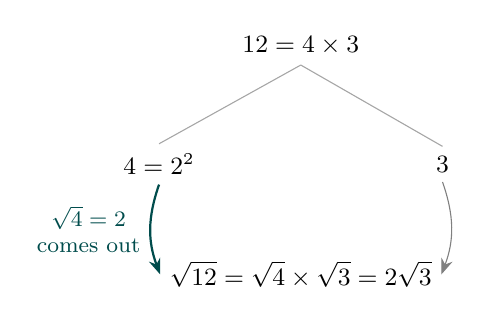
\begin{tikzpicture}[>={Stealth[length=2mm]},every node/.style={font=\small}]
\node (n) at (0,1.5) {$12=4\times 3$};
\node (sq) at (-1.8,0) {$4=2^{2}$};
\node (rem) at (1.8,0) {$3$};
\draw[gray!70] (n.south) -- (sq.north);
\draw[gray!70] (n.south) -- (rem.north);
\node (outc) at (0,-1.4) {$\displaystyle \sqrt{12}=\sqrt{4}\times\sqrt{3}=2\sqrt{3}$};
\draw[->,teal!60!black,thick] (sq.south) to[bend right=20] node[left,font=\footnotesize,align=center]{$\sqrt{4}=2$\\comes out} (outc.west);
\draw[->,gray] (rem.south) to[bend left=20] (outc.east);
\end{tikzpicture}
}
\end{center}
\small Factor tree: split the number into its largest perfect-square factor, then the square root of that factor comes out.\normalsize

\medskip\hrule

\section*{Laws of Surds 02\quad\small\texttt{(a5-002)}}
\addcontentsline{toc}{section}{Laws of Surds 02 (a5-002)}
\textit{Difficulty: Foundation \quad\textbar\quad Marks: 1}

\question{Simplify: \( \sqrt{18} \)}

\textbf{Worked solution.}

\textit{Step 1: Find the largest square number that is a factor of 18.}
\[\begin{gathered}
\sqrt{18} = \sqrt{9 \times 2}
\end{gathered}\]
9 is the largest square number that divides into 18.

\textit{Step 2: Split and simplify.}
\[\begin{gathered}
\sqrt{9} \times \sqrt{2} = 3\sqrt{2}
\end{gathered}\]
\( \sqrt{9} = 3 \).

\begin{answerbox}
\textbf{Final answer:}\quad \(\displaystyle 3\sqrt{2}\)
\end{answerbox}
\textbf{Diagram.}

\begin{center}
\resizebox{\ifdim\width>\linewidth \linewidth\else \width\fi}{!}{%
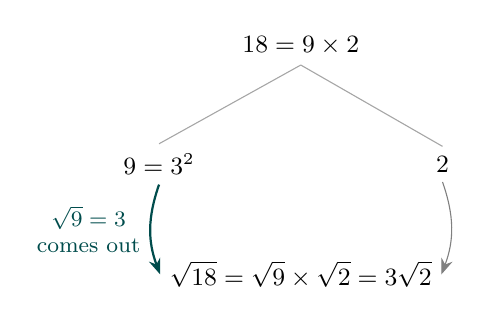
\begin{tikzpicture}[>={Stealth[length=2mm]},every node/.style={font=\small}]
\node (n) at (0,1.5) {$18=9\times 2$};
\node (sq) at (-1.8,0) {$9=3^{2}$};
\node (rem) at (1.8,0) {$2$};
\draw[gray!70] (n.south) -- (sq.north);
\draw[gray!70] (n.south) -- (rem.north);
\node (outc) at (0,-1.4) {$\displaystyle \sqrt{18}=\sqrt{9}\times\sqrt{2}=3\sqrt{2}$};
\draw[->,teal!60!black,thick] (sq.south) to[bend right=20] node[left,font=\footnotesize,align=center]{$\sqrt{9}=3$\\comes out} (outc.west);
\draw[->,gray] (rem.south) to[bend left=20] (outc.east);
\end{tikzpicture}
}
\end{center}
\small Factor tree: split the number into its largest perfect-square factor, then the square root of that factor comes out.\normalsize

\medskip\hrule

\section*{Laws of Surds 03\quad\small\texttt{(a5-003)}}
\addcontentsline{toc}{section}{Laws of Surds 03 (a5-003)}
\textit{Difficulty: Foundation \quad\textbar\quad Marks: 1}

\question{Simplify: \( \sqrt{45} \)}

\textbf{Worked solution.}

\textit{Step 1: Find the largest square number that is a factor of 45.}
\[\begin{gathered}
\sqrt{45} = \sqrt{9 \times 5}
\end{gathered}\]
9 is the largest square factor of 45.

\textit{Step 2: Split and simplify.}
\[\begin{gathered}
\sqrt{9} \times \sqrt{5} = 3\sqrt{5}
\end{gathered}\]
\( \sqrt{9} = 3 \).

\begin{answerbox}
\textbf{Final answer:}\quad \(\displaystyle 3\sqrt{5}\)
\end{answerbox}
\textbf{Diagram.}

\begin{center}
\resizebox{\ifdim\width>\linewidth \linewidth\else \width\fi}{!}{%
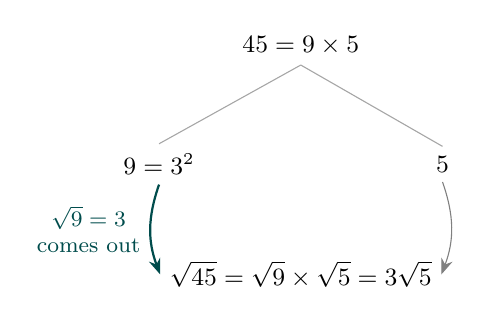
\begin{tikzpicture}[>={Stealth[length=2mm]},every node/.style={font=\small}]
\node (n) at (0,1.5) {$45=9\times 5$};
\node (sq) at (-1.8,0) {$9=3^{2}$};
\node (rem) at (1.8,0) {$5$};
\draw[gray!70] (n.south) -- (sq.north);
\draw[gray!70] (n.south) -- (rem.north);
\node (outc) at (0,-1.4) {$\displaystyle \sqrt{45}=\sqrt{9}\times\sqrt{5}=3\sqrt{5}$};
\draw[->,teal!60!black,thick] (sq.south) to[bend right=20] node[left,font=\footnotesize,align=center]{$\sqrt{9}=3$\\comes out} (outc.west);
\draw[->,gray] (rem.south) to[bend left=20] (outc.east);
\end{tikzpicture}
}
\end{center}
\small Factor tree: split the number into its largest perfect-square factor, then the square root of that factor comes out.\normalsize

\medskip\hrule

\section*{Laws of Surds 04\quad\small\texttt{(a5-004)}}
\addcontentsline{toc}{section}{Laws of Surds 04 (a5-004)}
\textit{Difficulty: Foundation \quad\textbar\quad Marks: 1}

\question{Simplify: \( \sqrt{75} \)}

\textbf{Worked solution.}

\textit{Step 1: Find the largest square number that is a factor of 75.}
\[\begin{gathered}
\sqrt{75} = \sqrt{25 \times 3}
\end{gathered}\]
25 is the largest square factor of 75.

\textit{Step 2: Split and simplify.}
\[\begin{gathered}
\sqrt{25} \times \sqrt{3} = 5\sqrt{3}
\end{gathered}\]
\( \sqrt{25} = 5 \).

\begin{answerbox}
\textbf{Final answer:}\quad \(\displaystyle 5\sqrt{3}\)
\end{answerbox}
\textbf{Diagram.}

\begin{center}
\resizebox{\ifdim\width>\linewidth \linewidth\else \width\fi}{!}{%
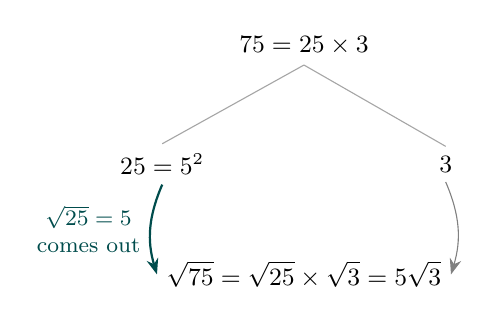
\begin{tikzpicture}[>={Stealth[length=2mm]},every node/.style={font=\small}]
\node (n) at (0,1.5) {$75=25\times 3$};
\node (sq) at (-1.8,0) {$25=5^{2}$};
\node (rem) at (1.8,0) {$3$};
\draw[gray!70] (n.south) -- (sq.north);
\draw[gray!70] (n.south) -- (rem.north);
\node (outc) at (0,-1.4) {$\displaystyle \sqrt{75}=\sqrt{25}\times\sqrt{3}=5\sqrt{3}$};
\draw[->,teal!60!black,thick] (sq.south) to[bend right=20] node[left,font=\footnotesize,align=center]{$\sqrt{25}=5$\\comes out} (outc.west);
\draw[->,gray] (rem.south) to[bend left=20] (outc.east);
\end{tikzpicture}
}
\end{center}
\small Factor tree: split the number into its largest perfect-square factor, then the square root of that factor comes out.\normalsize

\medskip\hrule

\section*{Laws of Surds 05\quad\small\texttt{(a5-005)}}
\addcontentsline{toc}{section}{Laws of Surds 05 (a5-005)}
\textit{Difficulty: Foundation \quad\textbar\quad Marks: 1}

\question{Simplify: \( \sqrt{98} \)}

\textbf{Worked solution.}

\textit{Step 1: Find the largest square number that is a factor of 98.}
\[\begin{gathered}
\sqrt{98} = \sqrt{49 \times 2}
\end{gathered}\]
49 is the largest square factor of 98.

\textit{Step 2: Split and simplify.}
\[\begin{gathered}
\sqrt{49} \times \sqrt{2} = 7\sqrt{2}
\end{gathered}\]
\( \sqrt{49} = 7 \).

\begin{answerbox}
\textbf{Final answer:}\quad \(\displaystyle 7\sqrt{2}\)
\end{answerbox}
\textbf{Diagram.}

\begin{center}
\resizebox{\ifdim\width>\linewidth \linewidth\else \width\fi}{!}{%
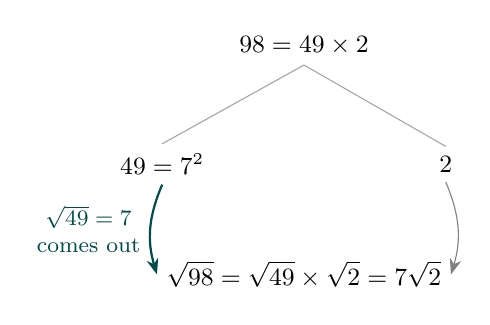
\begin{tikzpicture}[>={Stealth[length=2mm]},every node/.style={font=\small}]
\node (n) at (0,1.5) {$98=49\times 2$};
\node (sq) at (-1.8,0) {$49=7^{2}$};
\node (rem) at (1.8,0) {$2$};
\draw[gray!70] (n.south) -- (sq.north);
\draw[gray!70] (n.south) -- (rem.north);
\node (outc) at (0,-1.4) {$\displaystyle \sqrt{98}=\sqrt{49}\times\sqrt{2}=7\sqrt{2}$};
\draw[->,teal!60!black,thick] (sq.south) to[bend right=20] node[left,font=\footnotesize,align=center]{$\sqrt{49}=7$\\comes out} (outc.west);
\draw[->,gray] (rem.south) to[bend left=20] (outc.east);
\end{tikzpicture}
}
\end{center}
\small Factor tree: split the number into its largest perfect-square factor, then the square root of that factor comes out.\normalsize

\medskip\hrule

\section*{Laws of Surds 06\quad\small\texttt{(a5-006)}}
\addcontentsline{toc}{section}{Laws of Surds 06 (a5-006)}
\textit{Difficulty: Foundation \quad\textbar\quad Marks: 1}

\question{Simplify: \( \sqrt{\frac{7}{4}} \)}

\textbf{Worked solution.}

\textit{Step 1: Use the rule \( \sqrt{\frac{a}{b}} = \frac{\sqrt{a}}{\sqrt{b}} \).}
\[\begin{gathered}
\frac{\sqrt{7}}{\sqrt{4}}
\end{gathered}\]
Split the surd across the numerator and denominator.

\textit{Step 2: Simplify the denominator.}
\[\begin{gathered}
\frac{\sqrt{7}}{2}
\end{gathered}\]
\( \sqrt{4} = 2 \). The numerator \( \sqrt{7} \) cannot be simplified further.

\begin{answerbox}
\textbf{Final answer:}\quad \(\displaystyle \frac{\sqrt{7}}{2}\)
\end{answerbox}
\textbf{Diagram.}

\begin{center}
\resizebox{\ifdim\width>\linewidth \linewidth\else \width\fi}{!}{%
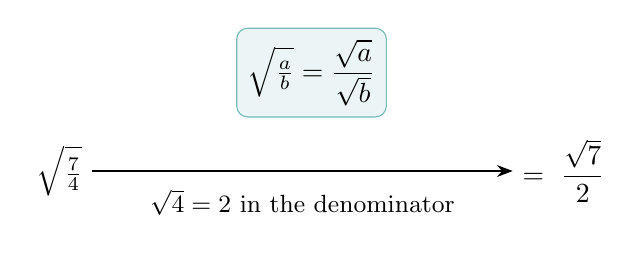
\begin{tikzpicture}[>={Stealth[length=2mm]}]
\node[draw=teal!55,rounded corners,fill=teal!8,inner sep=4pt] (rule) at (3.2,1.25) {$\displaystyle \sqrt{\tfrac{a}{b}}=\dfrac{\sqrt{a}}{\sqrt{b}}$};
\node (L) at (0,0) {$\displaystyle \sqrt{\tfrac{7}{4}}$};
\node (R) at (6.4,0) {$\displaystyle =\ \dfrac{\sqrt{7}}{2}$};
\draw[->,thick] (L) -- (R) node[midway,below=3pt,font=\small,align=center]{$\sqrt{4}=2$ in the denominator};
\end{tikzpicture}
}
\end{center}
\small Surd-law card: the boxed general rule (teal) is applied to the expression.\normalsize

\medskip\hrule

\section*{Laws of Surds 07\quad\small\texttt{(a5-007)}}
\addcontentsline{toc}{section}{Laws of Surds 07 (a5-007)}
\textit{Difficulty: Foundation \quad\textbar\quad Marks: 1}

\question{Simplify: \( \sqrt{\frac{9}{25}} \)}

\textbf{Worked solution.}

\textit{Step 1: Use the rule \( \sqrt{\frac{a}{b}} = \frac{\sqrt{a}}{\sqrt{b}} \).}
\[\begin{gathered}
\frac{\sqrt{9}}{\sqrt{25}}
\end{gathered}\]
Split the surd across the fraction.

\textit{Step 2: Evaluate both square roots.}
\[\begin{gathered}
\frac{3}{5}
\end{gathered}\]
\( \sqrt{9} = 3 \) and \( \sqrt{25} = 5 \). Both are perfect squares, so the answer is rational.

\begin{answerbox}
\textbf{Final answer:}\quad \(\displaystyle \frac{3}{5}\)
\end{answerbox}
\textbf{Diagram.}

\begin{center}
\resizebox{\ifdim\width>\linewidth \linewidth\else \width\fi}{!}{%
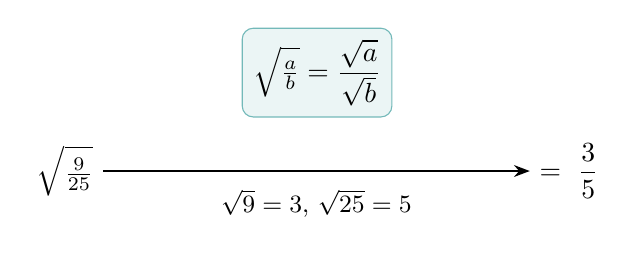
\begin{tikzpicture}[>={Stealth[length=2mm]}]
\node[draw=teal!55,rounded corners,fill=teal!8,inner sep=4pt] (rule) at (3.2,1.25) {$\displaystyle \sqrt{\tfrac{a}{b}}=\dfrac{\sqrt{a}}{\sqrt{b}}$};
\node (L) at (0,0) {$\displaystyle \sqrt{\tfrac{9}{25}}$};
\node (R) at (6.4,0) {$\displaystyle =\ \dfrac{3}{5}$};
\draw[->,thick] (L) -- (R) node[midway,below=3pt,font=\small,align=center]{$\sqrt{9}=3$, $\sqrt{25}=5$};
\end{tikzpicture}
}
\end{center}
\small Surd-law card: the boxed general rule (teal) is applied to the expression.\normalsize

\medskip\hrule

\section*{Laws of Surds 08\quad\small\texttt{(a5-008)}}
\addcontentsline{toc}{section}{Laws of Surds 08 (a5-008)}
\textit{Difficulty: Foundation \quad\textbar\quad Marks: 1}

\question{Simplify: \( \sqrt{\frac{11}{16}} \)}

\textbf{Worked solution.}

\textit{Step 1: Split the surd across the fraction.}
\[\begin{gathered}
\frac{\sqrt{11}}{\sqrt{16}}
\end{gathered}\]
\( \sqrt{\frac{a}{b}} = \frac{\sqrt{a}}{\sqrt{b}} \).

\textit{Step 2: Simplify the denominator.}
\[\begin{gathered}
\frac{\sqrt{11}}{4}
\end{gathered}\]
\( \sqrt{16} = 4 \). The numerator stays as \( \sqrt{11} \).

\begin{answerbox}
\textbf{Final answer:}\quad \(\displaystyle \frac{\sqrt{11}}{4}\)
\end{answerbox}
\textbf{Diagram.}

\begin{center}
\resizebox{\ifdim\width>\linewidth \linewidth\else \width\fi}{!}{%
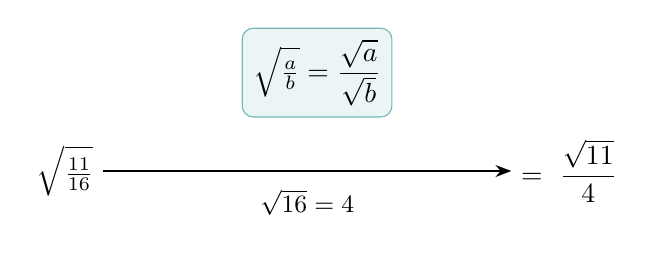
\begin{tikzpicture}[>={Stealth[length=2mm]}]
\node[draw=teal!55,rounded corners,fill=teal!8,inner sep=4pt] (rule) at (3.2,1.25) {$\displaystyle \sqrt{\tfrac{a}{b}}=\dfrac{\sqrt{a}}{\sqrt{b}}$};
\node (L) at (0,0) {$\displaystyle \sqrt{\tfrac{11}{16}}$};
\node (R) at (6.4,0) {$\displaystyle =\ \dfrac{\sqrt{11}}{4}$};
\draw[->,thick] (L) -- (R) node[midway,below=3pt,font=\small,align=center]{$\sqrt{16}=4$};
\end{tikzpicture}
}
\end{center}
\small Surd-law card: the boxed general rule (teal) is applied to the expression.\normalsize

\medskip\hrule

\section*{Laws of Surds 09\quad\small\texttt{(a5-009)}}
\addcontentsline{toc}{section}{Laws of Surds 09 (a5-009)}
\textit{Difficulty: Foundation \quad\textbar\quad Marks: 2}

\question{Evaluate: \( 3\sqrt{2} \times 5\sqrt{2} \). Give your answer as a whole number.}

\textbf{Worked solution.}

\textit{Step 1: Multiply the whole-number parts together and the surd parts together.}
\[\begin{gathered}
(3 \times 5) \times (\sqrt{2} \times \sqrt{2}) = 15 \times \sqrt{4}
\end{gathered}\]
Use the rule \( \sqrt{a} \times \sqrt{a} = a \).

\textit{Step 2: Simplify.}
\[\begin{gathered}
15 \times 2 = 30
\end{gathered}\]
\( \sqrt{2} \times \sqrt{2} = 2 \), so the surds disappear entirely.

\begin{answerbox}
\textbf{Final answer:}\quad \(\displaystyle 30\)
\end{answerbox}
\textbf{Diagram.}

\begin{center}
\resizebox{\ifdim\width>\linewidth \linewidth\else \width\fi}{!}{%
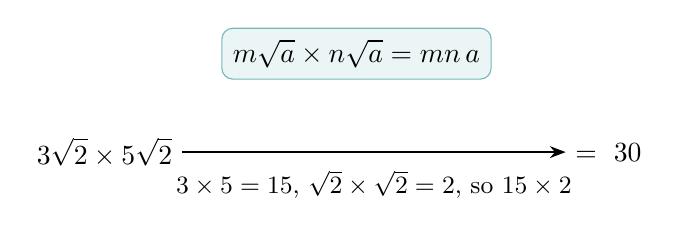
\begin{tikzpicture}[>={Stealth[length=2mm]}]
\node[draw=teal!55,rounded corners,fill=teal!8,inner sep=4pt] (rule) at (3.2,1.25) {$\displaystyle m\sqrt{a}\times n\sqrt{a}=mn\,a$};
\node (L) at (0,0) {$\displaystyle 3\sqrt{2}\times 5\sqrt{2}$};
\node (R) at (6.4,0) {$\displaystyle =\ 30$};
\draw[->,thick] (L) -- (R) node[midway,below=3pt,font=\small,align=center]{$3\times5=15$, $\sqrt2\times\sqrt2=2$, so $15\times2$};
\end{tikzpicture}
}
\end{center}
\small Surd-law card: the boxed general rule (teal) is applied to the expression.\normalsize

\medskip\hrule

\section*{Laws of Surds 10\quad\small\texttt{(a5-010)}}
\addcontentsline{toc}{section}{Laws of Surds 10 (a5-010)}
\textit{Difficulty: Foundation \quad\textbar\quad Marks: 1}

\question{Evaluate: \( \sqrt{6} \times \sqrt{6} \)}

\textbf{Worked solution.}

\textit{Apply the key rule \( (\sqrt{a})^2 = a \).}
\[\begin{gathered}
\sqrt{6} \times \sqrt{6} = 6
\end{gathered}\]
Squaring a surd removes the root sign. This follows directly from the definition of a square root.

\begin{answerbox}
\textbf{Final answer:}\quad \(\displaystyle 6\)
\end{answerbox}
\textbf{Diagram.}

\begin{center}
\resizebox{\ifdim\width>\linewidth \linewidth\else \width\fi}{!}{%
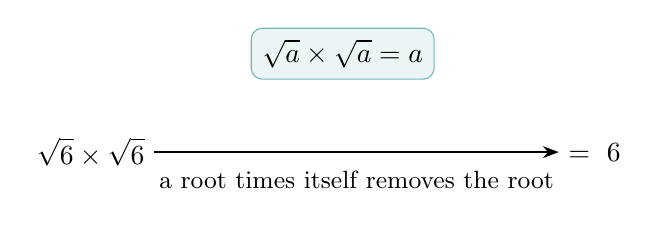
\begin{tikzpicture}[>={Stealth[length=2mm]}]
\node[draw=teal!55,rounded corners,fill=teal!8,inner sep=4pt] (rule) at (3.2,1.25) {$\displaystyle \sqrt{a}\times\sqrt{a}=a$};
\node (L) at (0,0) {$\displaystyle \sqrt{6}\times\sqrt{6}$};
\node (R) at (6.4,0) {$\displaystyle =\ 6$};
\draw[->,thick] (L) -- (R) node[midway,below=3pt,font=\small,align=center]{a root times itself removes the root};
\end{tikzpicture}
}
\end{center}
\small Surd-law card: the boxed general rule (teal) is applied to the expression.\normalsize

\medskip\hrule

\section*{Laws of Surds 11\quad\small\texttt{(a5-011)}}
\addcontentsline{toc}{section}{Laws of Surds 11 (a5-011)}
\textit{Difficulty: Foundation \quad\textbar\quad Marks: 1}

\question{Evaluate: \( \sqrt{3} \times 4\sqrt{3} \)}

\textbf{Worked solution.}

\textit{Multiply the surd parts and the number parts.}
\[\begin{gathered}
1 \times 4 \times (\sqrt{3} \times \sqrt{3}) = 4 \times 3 = 12
\end{gathered}\]
\( \sqrt{3} \times \sqrt{3} = 3 \), then multiply by 4.

\begin{answerbox}
\textbf{Final answer:}\quad \(\displaystyle 12\)
\end{answerbox}
\textbf{Diagram.}

\begin{center}
\resizebox{\ifdim\width>\linewidth \linewidth\else \width\fi}{!}{%
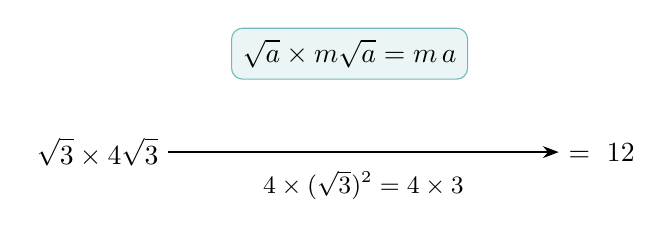
\begin{tikzpicture}[>={Stealth[length=2mm]}]
\node[draw=teal!55,rounded corners,fill=teal!8,inner sep=4pt] (rule) at (3.2,1.25) {$\displaystyle \sqrt{a}\times m\sqrt{a}=m\,a$};
\node (L) at (0,0) {$\displaystyle \sqrt{3}\times 4\sqrt{3}$};
\node (R) at (6.4,0) {$\displaystyle =\ 12$};
\draw[->,thick] (L) -- (R) node[midway,below=3pt,font=\small,align=center]{$4\times(\sqrt3)^2=4\times3$};
\end{tikzpicture}
}
\end{center}
\small Surd-law card: the boxed general rule (teal) is applied to the expression.\normalsize

\medskip\hrule

\section*{Laws of Surds 12\quad\small\texttt{(a5-012)}}
\addcontentsline{toc}{section}{Laws of Surds 12 (a5-012)}
\textit{Difficulty: Foundation \quad\textbar\quad Marks: 2}

\question{Evaluate: \( 2\sqrt{3} \times 4\sqrt{7} \). Give your answer as a surd.}

\textbf{Worked solution.}

\textit{Step 1: Multiply the whole-number parts together and the surd parts together.}
\[\begin{gathered}
(2 \times 4) \times (\sqrt{3} \times \sqrt{7})
\end{gathered}\]
Deal with the numbers and the surds separately.

\textit{Step 2: Simplify using \( \sqrt{a} \times \sqrt{b} = \sqrt{ab} \).}
\[\begin{gathered}
8\sqrt{21}
\end{gathered}\]
\( 2 \times 4 = 8 \) and \( \sqrt{3} \times \sqrt{7} = \sqrt{21} \). Since 21 has no square factors, this is fully simplified.

\begin{answerbox}
\textbf{Final answer:}\quad \(\displaystyle 8\sqrt{21}\)
\end{answerbox}
\textbf{Diagram.}

\begin{center}
\resizebox{\ifdim\width>\linewidth \linewidth\else \width\fi}{!}{%
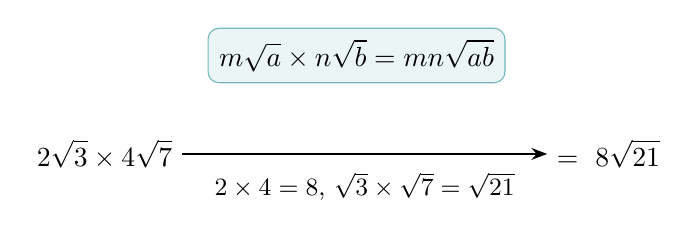
\begin{tikzpicture}[>={Stealth[length=2mm]}]
\node[draw=teal!55,rounded corners,fill=teal!8,inner sep=4pt] (rule) at (3.2,1.25) {$\displaystyle m\sqrt{a}\times n\sqrt{b}=mn\sqrt{ab}$};
\node (L) at (0,0) {$\displaystyle 2\sqrt{3}\times 4\sqrt{7}$};
\node (R) at (6.4,0) {$\displaystyle =\ 8\sqrt{21}$};
\draw[->,thick] (L) -- (R) node[midway,below=3pt,font=\small,align=center]{$2\times4=8$, $\sqrt3\times\sqrt7=\sqrt{21}$};
\end{tikzpicture}
}
\end{center}
\small Surd-law card: the boxed general rule (teal) is applied to the expression.\normalsize

\medskip\hrule

\section*{Laws of Surds 13\quad\small\texttt{(a5-013)}}
\addcontentsline{toc}{section}{Laws of Surds 13 (a5-013)}
\textit{Difficulty: Foundation \quad\textbar\quad Marks: 1}

\question{Evaluate: \( (\sqrt{5})^2 \)}

\textbf{Worked solution.}

\textit{Squaring a square root cancels out the root.}
\[\begin{gathered}
(\sqrt{5})^2 = 5
\end{gathered}\]
By definition, \( (\sqrt{a})^2 = a \). Squaring undoes the square root.

\begin{answerbox}
\textbf{Final answer:}\quad \(\displaystyle 5\)
\end{answerbox}
\textbf{Diagram.}

\begin{center}
\resizebox{\ifdim\width>\linewidth \linewidth\else \width\fi}{!}{%
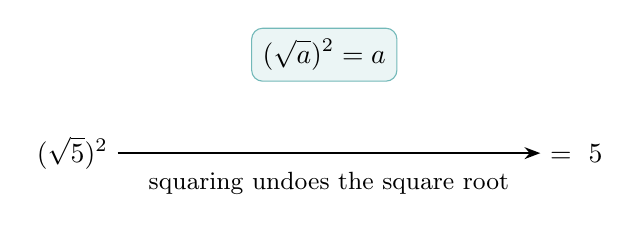
\begin{tikzpicture}[>={Stealth[length=2mm]}]
\node[draw=teal!55,rounded corners,fill=teal!8,inner sep=4pt] (rule) at (3.2,1.25) {$\displaystyle (\sqrt{a})^{2}=a$};
\node (L) at (0,0) {$\displaystyle (\sqrt{5})^{2}$};
\node (R) at (6.4,0) {$\displaystyle =\ 5$};
\draw[->,thick] (L) -- (R) node[midway,below=3pt,font=\small,align=center]{squaring undoes the square root};
\end{tikzpicture}
}
\end{center}
\small Surd-law card: the boxed general rule (teal) is applied to the expression.\normalsize

\medskip\hrule

\section*{Laws of Surds 14\quad\small\texttt{(a5-014)}}
\addcontentsline{toc}{section}{Laws of Surds 14 (a5-014)}
\textit{Difficulty: Foundation \quad\textbar\quad Marks: 2}

\question{Evaluate: \( (3\sqrt{7})^2 \)}

\textbf{Worked solution.}

\textit{Step 1: Square both the number part and the surd part.}
\[\begin{gathered}
3^2 \times (\sqrt{7})^2 = 9 \times 7
\end{gathered}\]
\( (a\sqrt{b})^2 = a^2 \times b \).

\textit{Step 2: Evaluate.}
\[\begin{gathered}
63
\end{gathered}\]
\( 9 \times 7 = 63 \).

\begin{answerbox}
\textbf{Final answer:}\quad \(\displaystyle 63\)
\end{answerbox}
\textbf{Diagram.}

\begin{center}
\resizebox{\ifdim\width>\linewidth \linewidth\else \width\fi}{!}{%
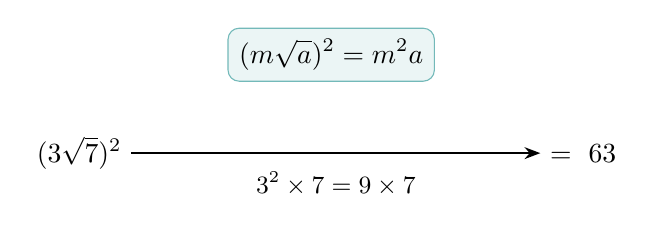
\begin{tikzpicture}[>={Stealth[length=2mm]}]
\node[draw=teal!55,rounded corners,fill=teal!8,inner sep=4pt] (rule) at (3.2,1.25) {$\displaystyle (m\sqrt{a})^{2}=m^{2}a$};
\node (L) at (0,0) {$\displaystyle (3\sqrt{7})^{2}$};
\node (R) at (6.4,0) {$\displaystyle =\ 63$};
\draw[->,thick] (L) -- (R) node[midway,below=3pt,font=\small,align=center]{$3^{2}\times7=9\times7$};
\end{tikzpicture}
}
\end{center}
\small Surd-law card: the boxed general rule (teal) is applied to the expression.\normalsize

\medskip\hrule

\section*{Laws of Surds 15\quad\small\texttt{(a5-015)}}
\addcontentsline{toc}{section}{Laws of Surds 15 (a5-015)}
\textit{Difficulty: Foundation \quad\textbar\quad Marks: 2}

\question{Evaluate: \( (2\sqrt{13})^2 \)}

\textbf{Worked solution.}

\textit{Step 1: Square the coefficient and the surd separately.}
\[\begin{gathered}
2^2 \times (\sqrt{13})^2 = 4 \times 13
\end{gathered}\]
The square of \( 2 \) is 4, and squaring \( \sqrt{13} \) gives 13.

\textit{Step 2: Evaluate.}
\[\begin{gathered}
52
\end{gathered}\]
\( 4 \times 13 = 52 \).

\begin{answerbox}
\textbf{Final answer:}\quad \(\displaystyle 52\)
\end{answerbox}
\textbf{Diagram.}

\begin{center}
\resizebox{\ifdim\width>\linewidth \linewidth\else \width\fi}{!}{%
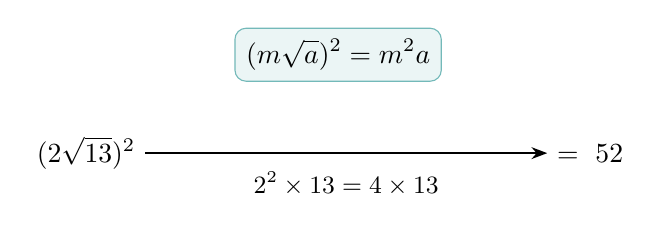
\begin{tikzpicture}[>={Stealth[length=2mm]}]
\node[draw=teal!55,rounded corners,fill=teal!8,inner sep=4pt] (rule) at (3.2,1.25) {$\displaystyle (m\sqrt{a})^{2}=m^{2}a$};
\node (L) at (0,0) {$\displaystyle (2\sqrt{13})^{2}$};
\node (R) at (6.4,0) {$\displaystyle =\ 52$};
\draw[->,thick] (L) -- (R) node[midway,below=3pt,font=\small,align=center]{$2^{2}\times13=4\times13$};
\end{tikzpicture}
}
\end{center}
\small Surd-law card: the boxed general rule (teal) is applied to the expression.\normalsize

\medskip\hrule

\section*{Laws of Surds 16\quad\small\texttt{(a5-016)}}
\addcontentsline{toc}{section}{Laws of Surds 16 (a5-016)}
\textit{Difficulty: Foundation \quad\textbar\quad Marks: 2}

\question{Evaluate: \( 3\sqrt{6} \times 2\sqrt{6} \)}

\textbf{Worked solution.}

\textit{Step 1: Multiply the coefficients and the surds separately.}
\[\begin{gathered}
(3 \times 2) \times (\sqrt{6} \times \sqrt{6}) = 6 \times 6
\end{gathered}\]
\( \sqrt{6} \times \sqrt{6} = 6 \).

\textit{Step 2: Evaluate.}
\[\begin{gathered}
36
\end{gathered}\]
\( 6 \times 6 = 36 \).

\begin{answerbox}
\textbf{Final answer:}\quad \(\displaystyle 36\)
\end{answerbox}
\textbf{Diagram.}

\begin{center}
\resizebox{\ifdim\width>\linewidth \linewidth\else \width\fi}{!}{%
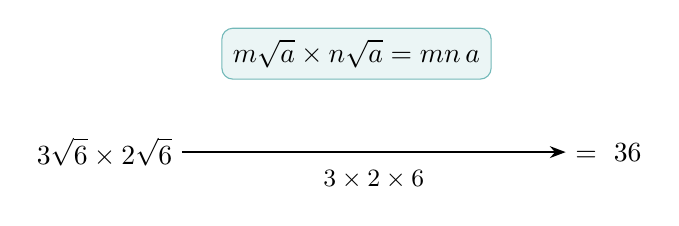
\begin{tikzpicture}[>={Stealth[length=2mm]}]
\node[draw=teal!55,rounded corners,fill=teal!8,inner sep=4pt] (rule) at (3.2,1.25) {$\displaystyle m\sqrt{a}\times n\sqrt{a}=mn\,a$};
\node (L) at (0,0) {$\displaystyle 3\sqrt{6}\times 2\sqrt{6}$};
\node (R) at (6.4,0) {$\displaystyle =\ 36$};
\draw[->,thick] (L) -- (R) node[midway,below=3pt,font=\small,align=center]{$3\times2\times6$};
\end{tikzpicture}
}
\end{center}
\small Surd-law card: the boxed general rule (teal) is applied to the expression.\normalsize

\medskip\hrule

\section*{Laws of Surds 17\quad\small\texttt{(a5-017)}}
\addcontentsline{toc}{section}{Laws of Surds 17 (a5-017)}
\textit{Difficulty: Foundation \quad\textbar\quad Marks: 2}

\question{Evaluate: \( 2\sqrt{3} \times 5\sqrt{27} \). Give your answer as a whole number.}

\textbf{Worked solution.}

\textit{Step 1: Multiply the coefficients and the surds separately.}
\[\begin{gathered}
(2 \times 5) \times (\sqrt{3} \times \sqrt{27}) = 10 \times \sqrt{81}
\end{gathered}\]
\( \sqrt{3} \times \sqrt{27} = \sqrt{3 \times 27} = \sqrt{81} \).

\textit{Step 2: Evaluate.}
\[\begin{gathered}
10 \times 9 = 90
\end{gathered}\]
\( \sqrt{81} = 9 \).

\begin{answerbox}
\textbf{Final answer:}\quad \(\displaystyle 90\)
\end{answerbox}
\textbf{Diagram.}

\begin{center}
\resizebox{\ifdim\width>\linewidth \linewidth\else \width\fi}{!}{%
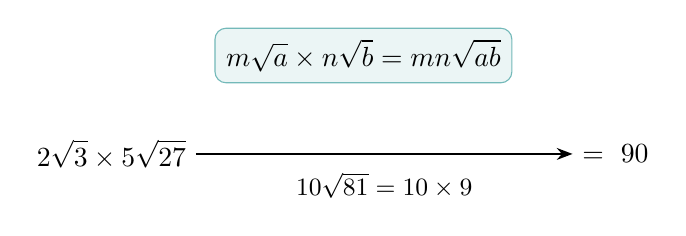
\begin{tikzpicture}[>={Stealth[length=2mm]}]
\node[draw=teal!55,rounded corners,fill=teal!8,inner sep=4pt] (rule) at (3.2,1.25) {$\displaystyle m\sqrt{a}\times n\sqrt{b}=mn\sqrt{ab}$};
\node (L) at (0,0) {$\displaystyle 2\sqrt{3}\times 5\sqrt{27}$};
\node (R) at (6.4,0) {$\displaystyle =\ 90$};
\draw[->,thick] (L) -- (R) node[midway,below=3pt,font=\small,align=center]{$10\sqrt{81}=10\times9$};
\end{tikzpicture}
}
\end{center}
\small Surd-law card: the boxed general rule (teal) is applied to the expression.\normalsize

\medskip\hrule

\section*{Laws of Surds 18\quad\small\texttt{(a5-018)}}
\addcontentsline{toc}{section}{Laws of Surds 18 (a5-018)}
\textit{Difficulty: Foundation \quad\textbar\quad Marks: 2}

\question{Evaluate: \( 3\sqrt{5} \times 2\sqrt{45} \). Give your answer as a whole number.}

\textbf{Worked solution.}

\textit{Step 1: Multiply the coefficients and the surds separately.}
\[\begin{gathered}
(3 \times 2) \times (\sqrt{5} \times \sqrt{45}) = 6 \times \sqrt{225}
\end{gathered}\]
\( \sqrt{5} \times \sqrt{45} = \sqrt{5 \times 45} = \sqrt{225} \).

\textit{Step 2: Evaluate.}
\[\begin{gathered}
6 \times 15 = 90
\end{gathered}\]
\( \sqrt{225} = 15 \).

\begin{answerbox}
\textbf{Final answer:}\quad \(\displaystyle 90\)
\end{answerbox}
\textbf{Diagram.}

\begin{center}
\resizebox{\ifdim\width>\linewidth \linewidth\else \width\fi}{!}{%
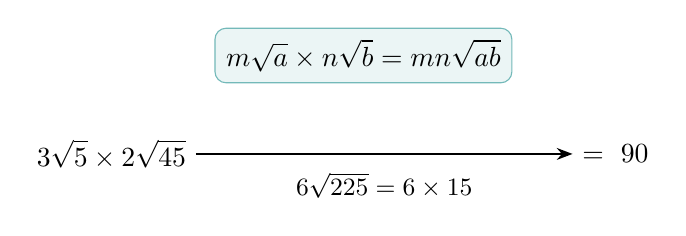
\begin{tikzpicture}[>={Stealth[length=2mm]}]
\node[draw=teal!55,rounded corners,fill=teal!8,inner sep=4pt] (rule) at (3.2,1.25) {$\displaystyle m\sqrt{a}\times n\sqrt{b}=mn\sqrt{ab}$};
\node (L) at (0,0) {$\displaystyle 3\sqrt{5}\times 2\sqrt{45}$};
\node (R) at (6.4,0) {$\displaystyle =\ 90$};
\draw[->,thick] (L) -- (R) node[midway,below=3pt,font=\small,align=center]{$6\sqrt{225}=6\times15$};
\end{tikzpicture}
}
\end{center}
\small Surd-law card: the boxed general rule (teal) is applied to the expression.\normalsize

\medskip\hrule

\section*{Laws of Surds 19\quad\small\texttt{(a5-019)}}
\addcontentsline{toc}{section}{Laws of Surds 19 (a5-019)}
\textit{Difficulty: Foundation \quad\textbar\quad Marks: 2}

\question{Evaluate: \( \frac{\sqrt{10}}{6} \times \frac{12}{\sqrt{5}} \)}

\textbf{Worked solution.}

\textit{Step 1: Multiply the fractions together.}
\[\begin{gathered}
\frac{12\sqrt{10}}{6\sqrt{5}}
\end{gathered}\]
Multiply numerators and denominators: \( \frac{\sqrt{10} \times 12}{6 \times \sqrt{5}} \).

\textit{Step 2: Simplify the number part and the surd part separately.}
\[\begin{gathered}
\frac{12}{6} \times \frac{\sqrt{10}}{\sqrt{5}} = 2 \times \sqrt{\frac{10}{5}} = 2\sqrt{2}
\end{gathered}\]
\( \frac{12}{6} = 2 \) and \( \frac{\sqrt{10}}{\sqrt{5}} = \sqrt{2} \).

\begin{answerbox}
\textbf{Final answer:}\quad \(\displaystyle 2\sqrt{2}\)
\end{answerbox}
\textbf{Diagram.}

\begin{center}
\resizebox{\ifdim\width>\linewidth \linewidth\else \width\fi}{!}{%
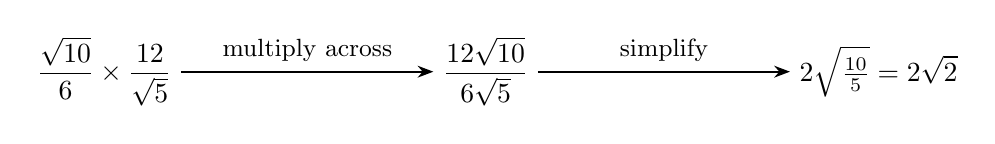
\begin{tikzpicture}[>={Stealth[length=2mm]},node distance=1.5cm and 3.2cm]
\node (s0) {$\displaystyle \frac{\sqrt{10}}{6}\times\frac{12}{\sqrt{5}}$};
\node (s1) [right=of s0] {$\displaystyle \frac{12\sqrt{10}}{6\sqrt{5}}$};
\node (s2) [right=of s1] {$\displaystyle 2\sqrt{\tfrac{10}{5}}=2\sqrt{2}$};
\draw[->,thick] (s0) -- (s1) node[midway,above,font=\small]{multiply across};
\draw[->,thick] (s1) -- (s2) node[midway,above,font=\small]{simplify};
\end{tikzpicture}
}
\end{center}
\small Solution flow: each arrow applies one surd law.\normalsize

\medskip\hrule

\section*{Laws of Surds 20\quad\small\texttt{(a5-020)}}
\addcontentsline{toc}{section}{Laws of Surds 20 (a5-020)}
\textit{Difficulty: Foundation \quad\textbar\quad Marks: 2}

\question{Evaluate: \( \frac{\sqrt{12}}{3} \times \frac{2}{\sqrt{27}} \)}

\textbf{Worked solution.}

\textit{Step 1: Multiply the fractions together.}
\[\begin{gathered}
\frac{2\sqrt{12}}{3\sqrt{27}}
\end{gathered}\]
Multiply the numerators and the denominators.

\textit{Step 2: Simplify the surd part.}
\[\begin{gathered}
\frac{2}{3} \times \sqrt{\frac{12}{27}} = \frac{2}{3} \times \sqrt{\frac{4}{9}} = \frac{2}{3} \times \frac{2}{3}
\end{gathered}\]
\( \frac{12}{27} = \frac{4}{9} \), and \( \sqrt{\frac{4}{9}} = \frac{2}{3} \).

\textit{Step 3: Evaluate.}
\[\begin{gathered}
\frac{4}{9}
\end{gathered}\]
\( \frac{2}{3} \times \frac{2}{3} = \frac{4}{9} \).

\begin{answerbox}
\textbf{Final answer:}\quad \(\displaystyle \frac{4}{9}\)
\end{answerbox}
\textbf{Diagram.}

\begin{center}
\resizebox{\ifdim\width>\linewidth \linewidth\else \width\fi}{!}{%
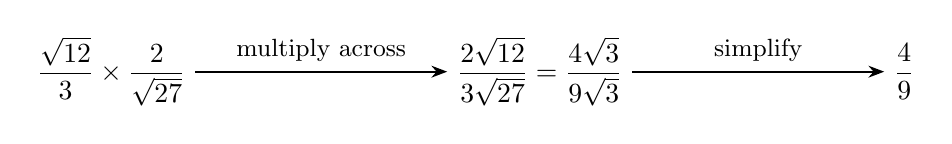
\begin{tikzpicture}[>={Stealth[length=2mm]},node distance=1.5cm and 3.2cm]
\node (s0) {$\displaystyle \frac{\sqrt{12}}{3}\times\frac{2}{\sqrt{27}}$};
\node (s1) [right=of s0] {$\displaystyle \frac{2\sqrt{12}}{3\sqrt{27}}=\frac{4\sqrt{3}}{9\sqrt{3}}$};
\node (s2) [right=of s1] {$\displaystyle \frac{4}{9}$};
\draw[->,thick] (s0) -- (s1) node[midway,above,font=\small]{multiply across};
\draw[->,thick] (s1) -- (s2) node[midway,above,font=\small]{simplify};
\end{tikzpicture}
}
\end{center}
\small Solution flow: each arrow applies one surd law.\normalsize

\medskip\hrule

\section*{Laws of Surds 21\quad\small\texttt{(a5-021)}}
\addcontentsline{toc}{section}{Laws of Surds 21 (a5-021)}
\textit{Difficulty: Foundation \quad\textbar\quad Marks: 2}

\question{Express \( \sqrt{48} + \sqrt{27} \) in the form \( k\sqrt{3} \), where \( k \) is an integer.}

\textbf{Worked solution.}

\textit{Step 1: Simplify each surd by finding the largest square factor.}
\[\begin{gathered}
\sqrt{48} = \sqrt{16 \times 3} = 4\sqrt{3} \quad \text{and} \quad \sqrt{27} = \sqrt{9 \times 3} = 3\sqrt{3}
\end{gathered}\]
16 is the largest square factor of 48, and 9 is the largest square factor of 27.

\textit{Step 2: Add the like surds.}
\[\begin{gathered}
4\sqrt{3} + 3\sqrt{3} = 7\sqrt{3}
\end{gathered}\]
These are like surds (both \( \sqrt{3} \)), so add the coefficients: \( 4 + 3 = 7 \).

\begin{answerbox}
\textbf{Final answer:}\quad \(\displaystyle 7\sqrt{3}\)
\end{answerbox}
\textbf{Diagram.}

\begin{center}
\resizebox{\ifdim\width>\linewidth \linewidth\else \width\fi}{!}{%
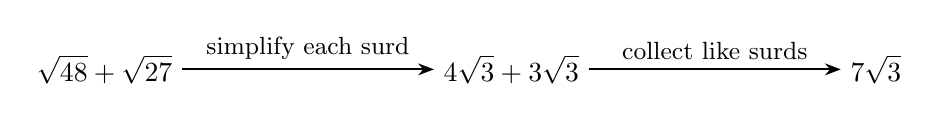
\begin{tikzpicture}[>={Stealth[length=2mm]},node distance=1.5cm and 3.2cm]
\node (s0) {$\displaystyle \sqrt{48}+\sqrt{27}$};
\node (s1) [right=of s0] {$\displaystyle 4\sqrt{3}+3\sqrt{3}$};
\node (s2) [right=of s1] {$\displaystyle 7\sqrt{3}$};
\draw[->,thick] (s0) -- (s1) node[midway,above,font=\small]{simplify each surd};
\draw[->,thick] (s1) -- (s2) node[midway,above,font=\small]{collect like surds};
\end{tikzpicture}
}
\end{center}
\small Solution flow: each arrow applies one surd law.\normalsize

\medskip\hrule

\section*{Laws of Surds 22\quad\small\texttt{(a5-022)}}
\addcontentsline{toc}{section}{Laws of Surds 22 (a5-022)}
\textit{Difficulty: Foundation \quad\textbar\quad Marks: 2}

\question{Express \( \sqrt{50} - \sqrt{8} \) in the form \( k\sqrt{2} \), where \( k \) is an integer.}

\textbf{Worked solution.}

\textit{Step 1: Simplify each surd.}
\[\begin{gathered}
\sqrt{50} = \sqrt{25 \times 2} = 5\sqrt{2} \quad \text{and} \quad \sqrt{8} = \sqrt{4 \times 2} = 2\sqrt{2}
\end{gathered}\]
25 is the largest square factor of 50, and 4 is the largest square factor of 8.

\textit{Step 2: Subtract the like surds.}
\[\begin{gathered}
5\sqrt{2} - 2\sqrt{2} = 3\sqrt{2}
\end{gathered}\]
Subtract the coefficients: \( 5 - 2 = 3 \).

\begin{answerbox}
\textbf{Final answer:}\quad \(\displaystyle 3\sqrt{2}\)
\end{answerbox}
\textbf{Diagram.}

\begin{center}
\resizebox{\ifdim\width>\linewidth \linewidth\else \width\fi}{!}{%
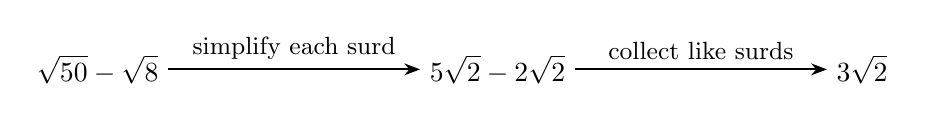
\begin{tikzpicture}[>={Stealth[length=2mm]},node distance=1.5cm and 3.2cm]
\node (s0) {$\displaystyle \sqrt{50}-\sqrt{8}$};
\node (s1) [right=of s0] {$\displaystyle 5\sqrt{2}-2\sqrt{2}$};
\node (s2) [right=of s1] {$\displaystyle 3\sqrt{2}$};
\draw[->,thick] (s0) -- (s1) node[midway,above,font=\small]{simplify each surd};
\draw[->,thick] (s1) -- (s2) node[midway,above,font=\small]{collect like surds};
\end{tikzpicture}
}
\end{center}
\small Solution flow: each arrow applies one surd law.\normalsize

\medskip\hrule

\section*{Laws of Surds 23\quad\small\texttt{(a5-023)}}
\addcontentsline{toc}{section}{Laws of Surds 23 (a5-023)}
\textit{Difficulty: Foundation \quad\textbar\quad Marks: 2}

\question{Express \( 3\sqrt{12} - 2\sqrt{75} \) in the form \( k\sqrt{3} \), where \( k \) is an integer.}

\textbf{Worked solution.}

\textit{Step 1: Simplify each surd.}
\[\begin{gathered}
3\sqrt{12} = 3 \times 2\sqrt{3} = 6\sqrt{3} \quad \text{and} \quad 2\sqrt{75} = 2 \times 5\sqrt{3} = 10\sqrt{3}
\end{gathered}\]
\( \sqrt{12} = 2\sqrt{3} \) and \( \sqrt{75} = 5\sqrt{3} \). Then multiply by the coefficients outside.

\textit{Step 2: Subtract the like surds.}
\[\begin{gathered}
6\sqrt{3} - 10\sqrt{3} = -4\sqrt{3}
\end{gathered}\]
\( 6 - 10 = -4 \). A negative answer is perfectly valid here.

\begin{answerbox}
\textbf{Final answer:}\quad \(\displaystyle -4\sqrt{3}\)
\end{answerbox}
\textbf{Diagram.}

\begin{center}
\resizebox{\ifdim\width>\linewidth \linewidth\else \width\fi}{!}{%
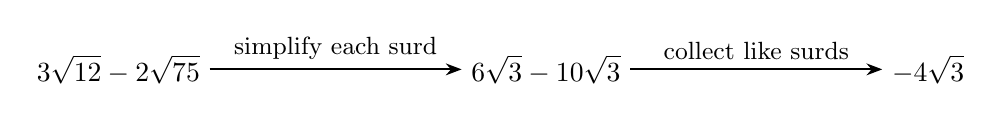
\begin{tikzpicture}[>={Stealth[length=2mm]},node distance=1.5cm and 3.2cm]
\node (s0) {$\displaystyle 3\sqrt{12}-2\sqrt{75}$};
\node (s1) [right=of s0] {$\displaystyle 6\sqrt{3}-10\sqrt{3}$};
\node (s2) [right=of s1] {$\displaystyle -4\sqrt{3}$};
\draw[->,thick] (s0) -- (s1) node[midway,above,font=\small]{simplify each surd};
\draw[->,thick] (s1) -- (s2) node[midway,above,font=\small]{collect like surds};
\end{tikzpicture}
}
\end{center}
\small Solution flow: each arrow applies one surd law.\normalsize

\medskip\hrule

\section*{Laws of Surds 24\quad\small\texttt{(a5-024)}}
\addcontentsline{toc}{section}{Laws of Surds 24 (a5-024)}
\textit{Difficulty: Foundation \quad\textbar\quad Marks: 2}

\question{Express \( 2\sqrt{18} + 3\sqrt{50} \) in the form \( k\sqrt{2} \), where \( k \) is an integer.}

\textbf{Worked solution.}

\textit{Step 1: Simplify each surd.}
\[\begin{gathered}
2\sqrt{18} = 2 \times 3\sqrt{2} = 6\sqrt{2} \quad \text{and} \quad 3\sqrt{50} = 3 \times 5\sqrt{2} = 15\sqrt{2}
\end{gathered}\]
\( \sqrt{18} = 3\sqrt{2} \) and \( \sqrt{50} = 5\sqrt{2} \).

\textit{Step 2: Add the like surds.}
\[\begin{gathered}
6\sqrt{2} + 15\sqrt{2} = 21\sqrt{2}
\end{gathered}\]
\( 6 + 15 = 21 \).

\begin{answerbox}
\textbf{Final answer:}\quad \(\displaystyle 21\sqrt{2}\)
\end{answerbox}
\textbf{Diagram.}

\begin{center}
\resizebox{\ifdim\width>\linewidth \linewidth\else \width\fi}{!}{%
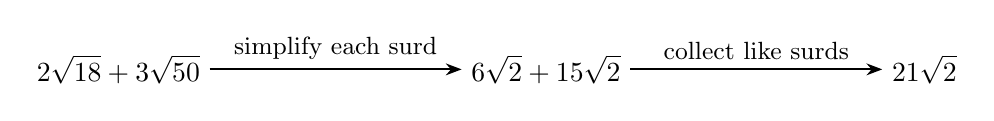
\begin{tikzpicture}[>={Stealth[length=2mm]},node distance=1.5cm and 3.2cm]
\node (s0) {$\displaystyle 2\sqrt{18}+3\sqrt{50}$};
\node (s1) [right=of s0] {$\displaystyle 6\sqrt{2}+15\sqrt{2}$};
\node (s2) [right=of s1] {$\displaystyle 21\sqrt{2}$};
\draw[->,thick] (s0) -- (s1) node[midway,above,font=\small]{simplify each surd};
\draw[->,thick] (s1) -- (s2) node[midway,above,font=\small]{collect like surds};
\end{tikzpicture}
}
\end{center}
\small Solution flow: each arrow applies one surd law.\normalsize

\medskip\hrule

\section*{Laws of Surds 25\quad\small\texttt{(a5-025)}}
\addcontentsline{toc}{section}{Laws of Surds 25 (a5-025)}
\textit{Difficulty: Foundation \quad\textbar\quad Marks: 3}

\question{Express \( 5\sqrt{28} + 3\sqrt{63} - 2\sqrt{7} \) in the form \( k\sqrt{7} \), where \( k \) is an integer.}

\textbf{Worked solution.}

\textit{Step 1: Simplify each surd.}
\[\begin{gathered}
5\sqrt{28} = 5 \times 2\sqrt{7} = 10\sqrt{7} \quad \text{and} \quad 3\sqrt{63} = 3 \times 3\sqrt{7} = 9\sqrt{7}
\end{gathered}\]
\( \sqrt{28} = 2\sqrt{7} \) and \( \sqrt{63} = 3\sqrt{7} \). The third term is already in surd form.

\textit{Step 2: Combine the like surds.}
\[\begin{gathered}
10\sqrt{7} + 9\sqrt{7} - 2\sqrt{7} = 17\sqrt{7}
\end{gathered}\]
\( 10 + 9 - 2 = 17 \).

\begin{answerbox}
\textbf{Final answer:}\quad \(\displaystyle 17\sqrt{7}\)
\end{answerbox}
\textbf{Diagram.}

\begin{center}
\resizebox{\ifdim\width>\linewidth \linewidth\else \width\fi}{!}{%
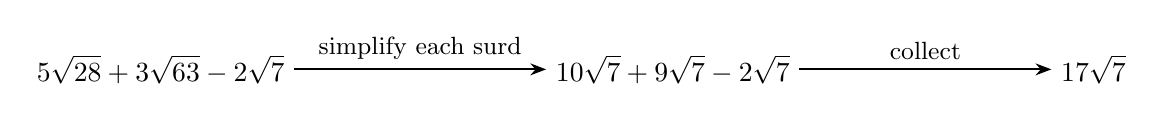
\begin{tikzpicture}[>={Stealth[length=2mm]},node distance=1.5cm and 3.2cm]
\node (s0) {$\displaystyle 5\sqrt{28}+3\sqrt{63}-2\sqrt{7}$};
\node (s1) [right=of s0] {$\displaystyle 10\sqrt{7}+9\sqrt{7}-2\sqrt{7}$};
\node (s2) [right=of s1] {$\displaystyle 17\sqrt{7}$};
\draw[->,thick] (s0) -- (s1) node[midway,above,font=\small]{simplify each surd};
\draw[->,thick] (s1) -- (s2) node[midway,above,font=\small]{collect};
\end{tikzpicture}
}
\end{center}
\small Solution flow: each arrow applies one surd law.\normalsize

\medskip\hrule

\section*{Laws of Surds 26\quad\small\texttt{(a5-026)}}
\addcontentsline{toc}{section}{Laws of Surds 26 (a5-026)}
\textit{Difficulty: Foundation \quad\textbar\quad Marks: 3}

\question{Express \( 2\sqrt{20} + 3\sqrt{45} + \sqrt{80} \) in the form \( k\sqrt{5} \), where \( k \) is an integer.}

\textbf{Worked solution.}

\textit{Step 1: Simplify each surd.}
\[\begin{gathered}
2\sqrt{20} = 2 \times 2\sqrt{5} = 4\sqrt{5}, \quad 3\sqrt{45} = 3 \times 3\sqrt{5} = 9\sqrt{5}, \quad \sqrt{80} = 4\sqrt{5}
\end{gathered}\]
\( \sqrt{20} = 2\sqrt{5} \), \( \sqrt{45} = 3\sqrt{5} \), and \( \sqrt{80} = \sqrt{16 \times 5} = 4\sqrt{5} \).

\textit{Step 2: Add the like surds.}
\[\begin{gathered}
4\sqrt{5} + 9\sqrt{5} + 4\sqrt{5} = 17\sqrt{5}
\end{gathered}\]
\( 4 + 9 + 4 = 17 \).

\begin{answerbox}
\textbf{Final answer:}\quad \(\displaystyle 17\sqrt{5}\)
\end{answerbox}
\textbf{Diagram.}

\begin{center}
\resizebox{\ifdim\width>\linewidth \linewidth\else \width\fi}{!}{%
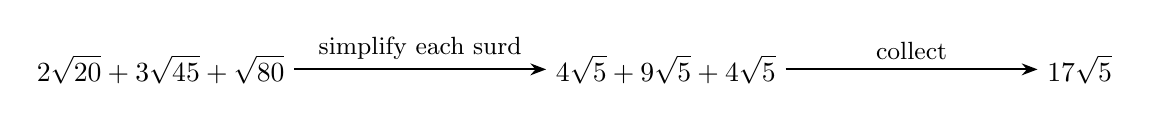
\begin{tikzpicture}[>={Stealth[length=2mm]},node distance=1.5cm and 3.2cm]
\node (s0) {$\displaystyle 2\sqrt{20}+3\sqrt{45}+\sqrt{80}$};
\node (s1) [right=of s0] {$\displaystyle 4\sqrt{5}+9\sqrt{5}+4\sqrt{5}$};
\node (s2) [right=of s1] {$\displaystyle 17\sqrt{5}$};
\draw[->,thick] (s0) -- (s1) node[midway,above,font=\small]{simplify each surd};
\draw[->,thick] (s1) -- (s2) node[midway,above,font=\small]{collect};
\end{tikzpicture}
}
\end{center}
\small Solution flow: each arrow applies one surd law.\normalsize

\medskip\hrule

\section*{Laws of Surds 27\quad\small\texttt{(a5-027)}}
\addcontentsline{toc}{section}{Laws of Surds 27 (a5-027)}
\textit{Difficulty: Foundation \quad\textbar\quad Marks: 3}

\question{Expand and simplify: \( (2 + \sqrt{3})(4 + \sqrt{3}) \)}

\textbf{Worked solution.}

\textit{Expand and simplify}
\[\begin{gathered}
\begin{aligned} (2+\sqrt{3})(4+\sqrt{3}) &= 2(4+\sqrt{3})+\sqrt{3}(4+\sqrt{3}) \\ &= 8+2\sqrt{3}+4\sqrt{3}+3 \\ &= 11 + 6\sqrt{3} \end{aligned}
\end{gathered}\]
Distribute each term in the first bracket across the second. Then collect rational parts (\(8+3=11\)) and surd parts (\(2\sqrt{3}+4\sqrt{3}=6\sqrt{3}\)).

\begin{answerbox}
\textbf{Final answer:}\quad \(\displaystyle 11 + 6\sqrt{3}\)
\end{answerbox}
\textbf{Diagram.}

\begin{center}
\resizebox{\ifdim\width>\linewidth \linewidth\else \width\fi}{!}{%
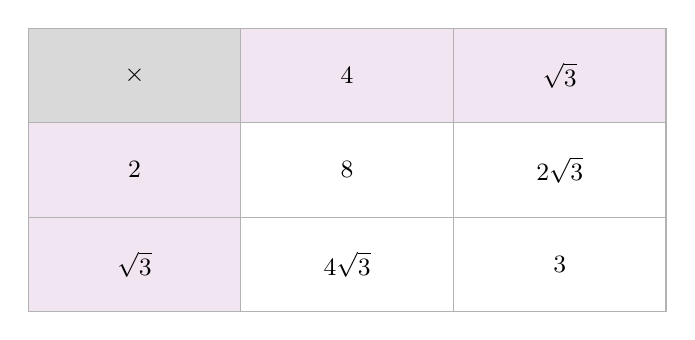
\begin{tikzpicture}[x=1cm,y=1cm,every node/.style={font=\small}]
\fill[gray!30] (0,0) rectangle (2.7,-1.2);
\draw[gray!60] (0,0) rectangle (2.7,-1.2);
\node at (1.35,-0.6) {$\displaystyle \times$};
\fill[violet!10] (2.7,0) rectangle (5.4,-1.2);
\draw[gray!60] (2.7,0) rectangle (5.4,-1.2);
\node at (4.05,-0.6) {$\displaystyle 4$};
\fill[violet!10] (5.4,0) rectangle (8.1,-1.2);
\draw[gray!60] (5.4,0) rectangle (8.1,-1.2);
\node at (6.75,-0.6) {$\displaystyle \sqrt{3}$};
\fill[violet!10] (0,-1.2) rectangle (2.7,-2.4);
\draw[gray!60] (0,-1.2) rectangle (2.7,-2.4);
\node at (1.35,-1.8) {$\displaystyle 2$};
\fill[white] (2.7,-1.2) rectangle (5.4,-2.4);
\draw[gray!60] (2.7,-1.2) rectangle (5.4,-2.4);
\node at (4.05,-1.8) {$\displaystyle 8$};
\fill[white] (5.4,-1.2) rectangle (8.1,-2.4);
\draw[gray!60] (5.4,-1.2) rectangle (8.1,-2.4);
\node at (6.75,-1.8) {$\displaystyle 2\sqrt{3}$};
\fill[violet!10] (0,-2.4) rectangle (2.7,-3.6);
\draw[gray!60] (0,-2.4) rectangle (2.7,-3.6);
\node at (1.35,-3) {$\displaystyle \sqrt{3}$};
\fill[white] (2.7,-2.4) rectangle (5.4,-3.6);
\draw[gray!60] (2.7,-2.4) rectangle (5.4,-3.6);
\node at (4.05,-3) {$\displaystyle 4\sqrt{3}$};
\fill[white] (5.4,-2.4) rectangle (8.1,-3.6);
\draw[gray!60] (5.4,-2.4) rectangle (8.1,-3.6);
\node at (6.75,-3) {$\displaystyle 3$};
\end{tikzpicture}
}
\end{center}
\small Collect: rational $8+3=11$; surd $2\sqrt3+4\sqrt3=6\sqrt3$. Area model (box method): the two binomial terms label the rows and columns; sum the cells, then collect the rational and surd parts.\normalsize

\medskip\hrule

\section*{Laws of Surds 28\quad\small\texttt{(a5-028)}}
\addcontentsline{toc}{section}{Laws of Surds 28 (a5-028)}
\textit{Difficulty: Foundation \quad\textbar\quad Marks: 3}

\question{Expand and simplify: \( (5 + 2\sqrt{7})(3 - \sqrt{7}) \)}

\textbf{Worked solution.}

\textit{Expand and simplify}
\[\begin{gathered}
\begin{aligned} (5+2\sqrt{7})(3-\sqrt{7}) &= 5(3-\sqrt{7})+2\sqrt{7}(3-\sqrt{7}) \\ &= 15-5\sqrt{7}+6\sqrt{7}-2(7) \\ &= 15-14-5\sqrt{7}+6\sqrt{7} \\ &= 1 + \sqrt{7} \end{aligned}
\end{gathered}\]
Distribute each term. Note \(2\sqrt{7} \times \sqrt{7} = 2 \times 7 = 14\). Then collect rational and surd parts.

\begin{answerbox}
\textbf{Final answer:}\quad \(\displaystyle 1 + \sqrt{7}\)
\end{answerbox}
\textbf{Diagram.}

\begin{center}
\resizebox{\ifdim\width>\linewidth \linewidth\else \width\fi}{!}{%
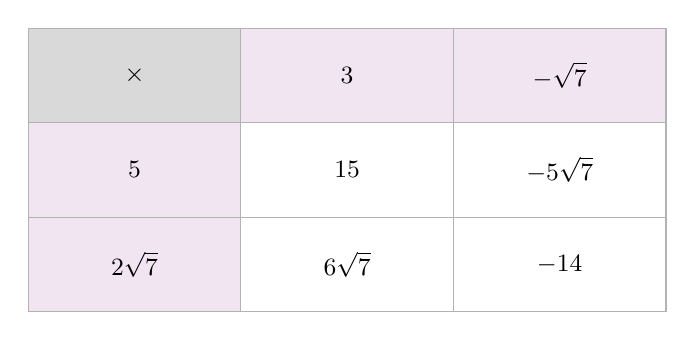
\begin{tikzpicture}[x=1cm,y=1cm,every node/.style={font=\small}]
\fill[gray!30] (0,0) rectangle (2.7,-1.2);
\draw[gray!60] (0,0) rectangle (2.7,-1.2);
\node at (1.35,-0.6) {$\displaystyle \times$};
\fill[violet!10] (2.7,0) rectangle (5.4,-1.2);
\draw[gray!60] (2.7,0) rectangle (5.4,-1.2);
\node at (4.05,-0.6) {$\displaystyle 3$};
\fill[violet!10] (5.4,0) rectangle (8.1,-1.2);
\draw[gray!60] (5.4,0) rectangle (8.1,-1.2);
\node at (6.75,-0.6) {$\displaystyle -\sqrt{7}$};
\fill[violet!10] (0,-1.2) rectangle (2.7,-2.4);
\draw[gray!60] (0,-1.2) rectangle (2.7,-2.4);
\node at (1.35,-1.8) {$\displaystyle 5$};
\fill[white] (2.7,-1.2) rectangle (5.4,-2.4);
\draw[gray!60] (2.7,-1.2) rectangle (5.4,-2.4);
\node at (4.05,-1.8) {$\displaystyle 15$};
\fill[white] (5.4,-1.2) rectangle (8.1,-2.4);
\draw[gray!60] (5.4,-1.2) rectangle (8.1,-2.4);
\node at (6.75,-1.8) {$\displaystyle -5\sqrt{7}$};
\fill[violet!10] (0,-2.4) rectangle (2.7,-3.6);
\draw[gray!60] (0,-2.4) rectangle (2.7,-3.6);
\node at (1.35,-3) {$\displaystyle 2\sqrt{7}$};
\fill[white] (2.7,-2.4) rectangle (5.4,-3.6);
\draw[gray!60] (2.7,-2.4) rectangle (5.4,-3.6);
\node at (4.05,-3) {$\displaystyle 6\sqrt{7}$};
\fill[white] (5.4,-2.4) rectangle (8.1,-3.6);
\draw[gray!60] (5.4,-2.4) rectangle (8.1,-3.6);
\node at (6.75,-3) {$\displaystyle -14$};
\end{tikzpicture}
}
\end{center}
\small Collect: $15-14=1$; $-5\sqrt7+6\sqrt7=\sqrt7$. Note $2\sqrt7\times(-\sqrt7)=-2\times7=-14$. Area model (box method): the two binomial terms label the rows and columns; sum the cells, then collect the rational and surd parts.\normalsize

\medskip\hrule

\section*{Laws of Surds 29\quad\small\texttt{(a5-029)}}
\addcontentsline{toc}{section}{Laws of Surds 29 (a5-029)}
\textit{Difficulty: Foundation \quad\textbar\quad Marks: 3}

\question{Expand and simplify: \( (\sqrt{5} + 3)(\sqrt{5} - 1) \)}

\textbf{Worked solution.}

\textit{Expand and simplify}
\[\begin{gathered}
\begin{aligned} (\sqrt{5}+3)(\sqrt{5}-1) &= \sqrt{5}(\sqrt{5}-1)+3(\sqrt{5}-1) \\ &= 5-\sqrt{5}+3\sqrt{5}-3 \\ &= 2 + 2\sqrt{5} \end{aligned}
\end{gathered}\]
Distribute each term. Rational parts: \(5-3=2\). Surd parts: \(-\sqrt{5}+3\sqrt{5}=2\sqrt{5}\).

\begin{answerbox}
\textbf{Final answer:}\quad \(\displaystyle 2 + 2\sqrt{5}\)
\end{answerbox}
\textbf{Diagram.}

\begin{center}
\resizebox{\ifdim\width>\linewidth \linewidth\else \width\fi}{!}{%
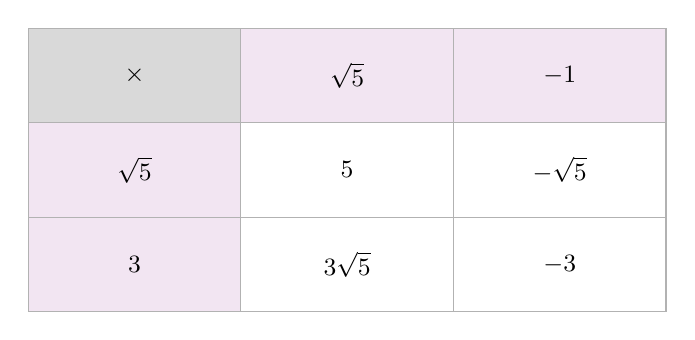
\begin{tikzpicture}[x=1cm,y=1cm,every node/.style={font=\small}]
\fill[gray!30] (0,0) rectangle (2.7,-1.2);
\draw[gray!60] (0,0) rectangle (2.7,-1.2);
\node at (1.35,-0.6) {$\displaystyle \times$};
\fill[violet!10] (2.7,0) rectangle (5.4,-1.2);
\draw[gray!60] (2.7,0) rectangle (5.4,-1.2);
\node at (4.05,-0.6) {$\displaystyle \sqrt{5}$};
\fill[violet!10] (5.4,0) rectangle (8.1,-1.2);
\draw[gray!60] (5.4,0) rectangle (8.1,-1.2);
\node at (6.75,-0.6) {$\displaystyle -1$};
\fill[violet!10] (0,-1.2) rectangle (2.7,-2.4);
\draw[gray!60] (0,-1.2) rectangle (2.7,-2.4);
\node at (1.35,-1.8) {$\displaystyle \sqrt{5}$};
\fill[white] (2.7,-1.2) rectangle (5.4,-2.4);
\draw[gray!60] (2.7,-1.2) rectangle (5.4,-2.4);
\node at (4.05,-1.8) {$\displaystyle 5$};
\fill[white] (5.4,-1.2) rectangle (8.1,-2.4);
\draw[gray!60] (5.4,-1.2) rectangle (8.1,-2.4);
\node at (6.75,-1.8) {$\displaystyle -\sqrt{5}$};
\fill[violet!10] (0,-2.4) rectangle (2.7,-3.6);
\draw[gray!60] (0,-2.4) rectangle (2.7,-3.6);
\node at (1.35,-3) {$\displaystyle 3$};
\fill[white] (2.7,-2.4) rectangle (5.4,-3.6);
\draw[gray!60] (2.7,-2.4) rectangle (5.4,-3.6);
\node at (4.05,-3) {$\displaystyle 3\sqrt{5}$};
\fill[white] (5.4,-2.4) rectangle (8.1,-3.6);
\draw[gray!60] (5.4,-2.4) rectangle (8.1,-3.6);
\node at (6.75,-3) {$\displaystyle -3$};
\end{tikzpicture}
}
\end{center}
\small Collect: $5-3=2$; $-\sqrt5+3\sqrt5=2\sqrt5$. Area model (box method): the two binomial terms label the rows and columns; sum the cells, then collect the rational and surd parts.\normalsize

\medskip\hrule

\section*{Laws of Surds 30\quad\small\texttt{(a5-030)}}
\addcontentsline{toc}{section}{Laws of Surds 30 (a5-030)}
\textit{Difficulty: Foundation \quad\textbar\quad Marks: 2}

\question{Expand and simplify: \( (\sqrt{11} + 3)(\sqrt{11} - 3) \)}

\textbf{Worked solution.}

\textit{Step 1: Recognise this as the difference of two squares pattern: \( (\sqrt{a} + b)(\sqrt{a} - b) = a - b^2 \).}
\[\begin{gathered}
(\sqrt{11})^2 - 3^2
\end{gathered}\]
The two brackets are conjugates — one has a plus, the other has a minus — so the middle surd terms cancel.

\textit{Step 2: Evaluate.}
\[\begin{gathered}
11 - 9 = 2
\end{gathered}\]
The result is a rational number with no surds remaining. This is the key idea behind rationalising denominators.

\begin{answerbox}
\textbf{Final answer:}\quad \(\displaystyle 2\)
\end{answerbox}
\textbf{Diagram.}

\begin{center}
\resizebox{\ifdim\width>\linewidth \linewidth\else \width\fi}{!}{%
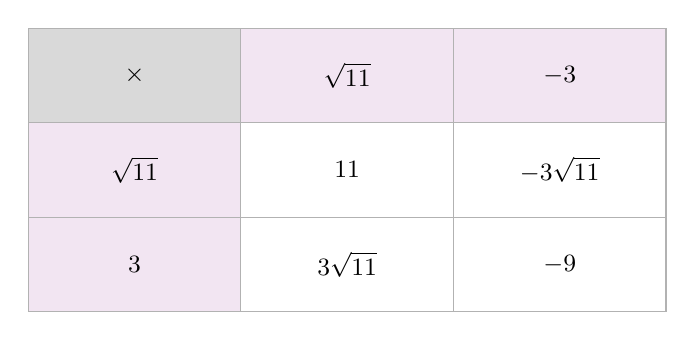
\begin{tikzpicture}[x=1cm,y=1cm,every node/.style={font=\small}]
\fill[gray!30] (0,0) rectangle (2.7,-1.2);
\draw[gray!60] (0,0) rectangle (2.7,-1.2);
\node at (1.35,-0.6) {$\displaystyle \times$};
\fill[violet!10] (2.7,0) rectangle (5.4,-1.2);
\draw[gray!60] (2.7,0) rectangle (5.4,-1.2);
\node at (4.05,-0.6) {$\displaystyle \sqrt{11}$};
\fill[violet!10] (5.4,0) rectangle (8.1,-1.2);
\draw[gray!60] (5.4,0) rectangle (8.1,-1.2);
\node at (6.75,-0.6) {$\displaystyle -3$};
\fill[violet!10] (0,-1.2) rectangle (2.7,-2.4);
\draw[gray!60] (0,-1.2) rectangle (2.7,-2.4);
\node at (1.35,-1.8) {$\displaystyle \sqrt{11}$};
\fill[white] (2.7,-1.2) rectangle (5.4,-2.4);
\draw[gray!60] (2.7,-1.2) rectangle (5.4,-2.4);
\node at (4.05,-1.8) {$\displaystyle 11$};
\fill[white] (5.4,-1.2) rectangle (8.1,-2.4);
\draw[gray!60] (5.4,-1.2) rectangle (8.1,-2.4);
\node at (6.75,-1.8) {$\displaystyle -3\sqrt{11}$};
\fill[violet!10] (0,-2.4) rectangle (2.7,-3.6);
\draw[gray!60] (0,-2.4) rectangle (2.7,-3.6);
\node at (1.35,-3) {$\displaystyle 3$};
\fill[white] (2.7,-2.4) rectangle (5.4,-3.6);
\draw[gray!60] (2.7,-2.4) rectangle (5.4,-3.6);
\node at (4.05,-3) {$\displaystyle 3\sqrt{11}$};
\fill[white] (5.4,-2.4) rectangle (8.1,-3.6);
\draw[gray!60] (5.4,-2.4) rectangle (8.1,-3.6);
\node at (6.75,-3) {$\displaystyle -9$};
\end{tikzpicture}
}
\end{center}
\small Difference of two squares: the surd cross-terms cancel, leaving $11-9=2$. Area model (box method): the two binomial terms label the rows and columns; sum the cells, then collect the rational and surd parts.\normalsize

\medskip\hrule

\section*{Laws of Surds 31\quad\small\texttt{(a5-031)}}
\addcontentsline{toc}{section}{Laws of Surds 31 (a5-031)}
\textit{Difficulty: Foundation \quad\textbar\quad Marks: 2}

\question{Expand and simplify: \( (7 - 2\sqrt{3})(7 + 2\sqrt{3}) \)}

\textbf{Worked solution.}

\textit{Step 1: Apply the difference of two squares: \( (a - b)(a + b) = a^2 - b^2 \).}
\[\begin{gathered}
7^2 - (2\sqrt{3})^2
\end{gathered}\]
These are conjugate pairs, so the cross terms cancel.

\textit{Step 2: Evaluate each square.}
\[\begin{gathered}
49 - 4 \times 3 = 49 - 12 = 37
\end{gathered}\]
\( (2\sqrt{3})^2 = 4 \times 3 = 12 \).

\begin{answerbox}
\textbf{Final answer:}\quad \(\displaystyle 37\)
\end{answerbox}
\textbf{Diagram.}

\begin{center}
\resizebox{\ifdim\width>\linewidth \linewidth\else \width\fi}{!}{%
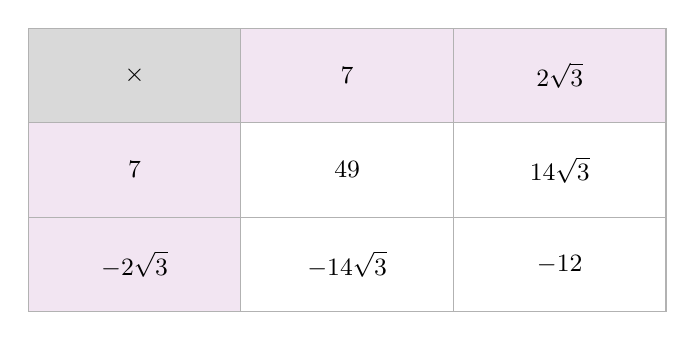
\begin{tikzpicture}[x=1cm,y=1cm,every node/.style={font=\small}]
\fill[gray!30] (0,0) rectangle (2.7,-1.2);
\draw[gray!60] (0,0) rectangle (2.7,-1.2);
\node at (1.35,-0.6) {$\displaystyle \times$};
\fill[violet!10] (2.7,0) rectangle (5.4,-1.2);
\draw[gray!60] (2.7,0) rectangle (5.4,-1.2);
\node at (4.05,-0.6) {$\displaystyle 7$};
\fill[violet!10] (5.4,0) rectangle (8.1,-1.2);
\draw[gray!60] (5.4,0) rectangle (8.1,-1.2);
\node at (6.75,-0.6) {$\displaystyle 2\sqrt{3}$};
\fill[violet!10] (0,-1.2) rectangle (2.7,-2.4);
\draw[gray!60] (0,-1.2) rectangle (2.7,-2.4);
\node at (1.35,-1.8) {$\displaystyle 7$};
\fill[white] (2.7,-1.2) rectangle (5.4,-2.4);
\draw[gray!60] (2.7,-1.2) rectangle (5.4,-2.4);
\node at (4.05,-1.8) {$\displaystyle 49$};
\fill[white] (5.4,-1.2) rectangle (8.1,-2.4);
\draw[gray!60] (5.4,-1.2) rectangle (8.1,-2.4);
\node at (6.75,-1.8) {$\displaystyle 14\sqrt{3}$};
\fill[violet!10] (0,-2.4) rectangle (2.7,-3.6);
\draw[gray!60] (0,-2.4) rectangle (2.7,-3.6);
\node at (1.35,-3) {$\displaystyle -2\sqrt{3}$};
\fill[white] (2.7,-2.4) rectangle (5.4,-3.6);
\draw[gray!60] (2.7,-2.4) rectangle (5.4,-3.6);
\node at (4.05,-3) {$\displaystyle -14\sqrt{3}$};
\fill[white] (5.4,-2.4) rectangle (8.1,-3.6);
\draw[gray!60] (5.4,-2.4) rectangle (8.1,-3.6);
\node at (6.75,-3) {$\displaystyle -12$};
\end{tikzpicture}
}
\end{center}
\small DOTS: cross-terms cancel; $(2\sqrt3)^2=4\times3=12$, so $49-12=37$. Area model (box method): the two binomial terms label the rows and columns; sum the cells, then collect the rational and surd parts.\normalsize

\medskip\hrule

\section*{Laws of Surds 32\quad\small\texttt{(a5-032)}}
\addcontentsline{toc}{section}{Laws of Surds 32 (a5-032)}
\textit{Difficulty: Foundation \quad\textbar\quad Marks: 3}

\question{Expand and simplify: \( (\sqrt{3} + 2)^2 \)}

\textbf{Worked solution.}

\textit{Expand and simplify}
\[\begin{gathered}
\begin{aligned} (\sqrt{3}+2)^2 &= (\sqrt{3}+2)(\sqrt{3}+2) \\ &= \sqrt{3}(\sqrt{3}+2)+2(\sqrt{3}+2) \\ &= 3+2\sqrt{3}+2\sqrt{3}+4 \\ &= 7 + 4\sqrt{3} \end{aligned}
\end{gathered}\]
Write the square as two identical brackets, then distribute each term.

\begin{answerbox}
\textbf{Final answer:}\quad \(\displaystyle 7 + 4\sqrt{3}\)
\end{answerbox}
\textbf{Diagram.}

\begin{center}
\resizebox{\ifdim\width>\linewidth \linewidth\else \width\fi}{!}{%
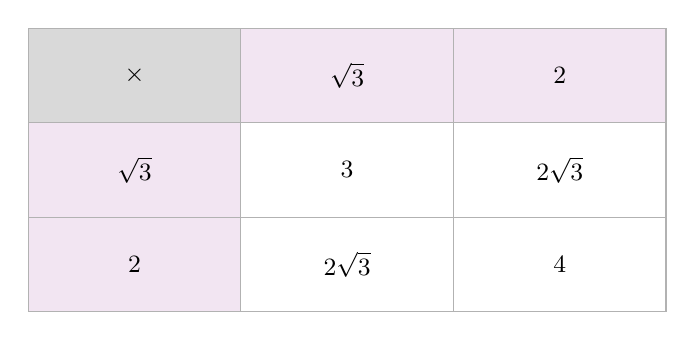
\begin{tikzpicture}[x=1cm,y=1cm,every node/.style={font=\small}]
\fill[gray!30] (0,0) rectangle (2.7,-1.2);
\draw[gray!60] (0,0) rectangle (2.7,-1.2);
\node at (1.35,-0.6) {$\displaystyle \times$};
\fill[violet!10] (2.7,0) rectangle (5.4,-1.2);
\draw[gray!60] (2.7,0) rectangle (5.4,-1.2);
\node at (4.05,-0.6) {$\displaystyle \sqrt{3}$};
\fill[violet!10] (5.4,0) rectangle (8.1,-1.2);
\draw[gray!60] (5.4,0) rectangle (8.1,-1.2);
\node at (6.75,-0.6) {$\displaystyle 2$};
\fill[violet!10] (0,-1.2) rectangle (2.7,-2.4);
\draw[gray!60] (0,-1.2) rectangle (2.7,-2.4);
\node at (1.35,-1.8) {$\displaystyle \sqrt{3}$};
\fill[white] (2.7,-1.2) rectangle (5.4,-2.4);
\draw[gray!60] (2.7,-1.2) rectangle (5.4,-2.4);
\node at (4.05,-1.8) {$\displaystyle 3$};
\fill[white] (5.4,-1.2) rectangle (8.1,-2.4);
\draw[gray!60] (5.4,-1.2) rectangle (8.1,-2.4);
\node at (6.75,-1.8) {$\displaystyle 2\sqrt{3}$};
\fill[violet!10] (0,-2.4) rectangle (2.7,-3.6);
\draw[gray!60] (0,-2.4) rectangle (2.7,-3.6);
\node at (1.35,-3) {$\displaystyle 2$};
\fill[white] (2.7,-2.4) rectangle (5.4,-3.6);
\draw[gray!60] (2.7,-2.4) rectangle (5.4,-3.6);
\node at (4.05,-3) {$\displaystyle 2\sqrt{3}$};
\fill[white] (5.4,-2.4) rectangle (8.1,-3.6);
\draw[gray!60] (5.4,-2.4) rectangle (8.1,-3.6);
\node at (6.75,-3) {$\displaystyle 4$};
\end{tikzpicture}
}
\end{center}
\small Perfect square: $3+4=7$ and $2\sqrt3+2\sqrt3=4\sqrt3$. Area model (box method): the two binomial terms label the rows and columns; sum the cells, then collect the rational and surd parts.\normalsize

\medskip\hrule

\section*{Laws of Surds 33\quad\small\texttt{(a5-033)}}
\addcontentsline{toc}{section}{Laws of Surds 33 (a5-033)}
\textit{Difficulty: Foundation \quad\textbar\quad Marks: 3}

\question{Expand and simplify: \( (2\sqrt{5} - 3)^2 \)}

\textbf{Worked solution.}

\textit{Expand and simplify}
\[\begin{gathered}
\begin{aligned} (2\sqrt{5}-3)^2 &= (2\sqrt{5}-3)(2\sqrt{5}-3) \\ &= 2\sqrt{5}(2\sqrt{5}-3)-3(2\sqrt{5}-3) \\ &= 4(5)-6\sqrt{5}-6\sqrt{5}+9 \\ &= 20-12\sqrt{5}+9 \\ &= 29 - 12\sqrt{5} \end{aligned}
\end{gathered}\]
Write the square as two identical brackets, then distribute each term. Note \(2\sqrt{5} \times 2\sqrt{5} = 4 \times 5 = 20\).

\begin{answerbox}
\textbf{Final answer:}\quad \(\displaystyle 29 - 12\sqrt{5}\)
\end{answerbox}
\textbf{Diagram.}

\begin{center}
\resizebox{\ifdim\width>\linewidth \linewidth\else \width\fi}{!}{%
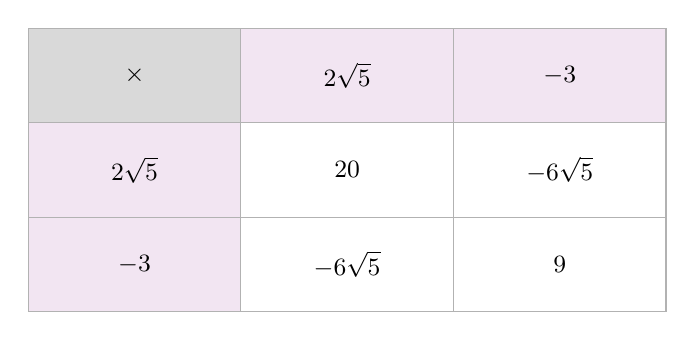
\begin{tikzpicture}[x=1cm,y=1cm,every node/.style={font=\small}]
\fill[gray!30] (0,0) rectangle (2.7,-1.2);
\draw[gray!60] (0,0) rectangle (2.7,-1.2);
\node at (1.35,-0.6) {$\displaystyle \times$};
\fill[violet!10] (2.7,0) rectangle (5.4,-1.2);
\draw[gray!60] (2.7,0) rectangle (5.4,-1.2);
\node at (4.05,-0.6) {$\displaystyle 2\sqrt{5}$};
\fill[violet!10] (5.4,0) rectangle (8.1,-1.2);
\draw[gray!60] (5.4,0) rectangle (8.1,-1.2);
\node at (6.75,-0.6) {$\displaystyle -3$};
\fill[violet!10] (0,-1.2) rectangle (2.7,-2.4);
\draw[gray!60] (0,-1.2) rectangle (2.7,-2.4);
\node at (1.35,-1.8) {$\displaystyle 2\sqrt{5}$};
\fill[white] (2.7,-1.2) rectangle (5.4,-2.4);
\draw[gray!60] (2.7,-1.2) rectangle (5.4,-2.4);
\node at (4.05,-1.8) {$\displaystyle 20$};
\fill[white] (5.4,-1.2) rectangle (8.1,-2.4);
\draw[gray!60] (5.4,-1.2) rectangle (8.1,-2.4);
\node at (6.75,-1.8) {$\displaystyle -6\sqrt{5}$};
\fill[violet!10] (0,-2.4) rectangle (2.7,-3.6);
\draw[gray!60] (0,-2.4) rectangle (2.7,-3.6);
\node at (1.35,-3) {$\displaystyle -3$};
\fill[white] (2.7,-2.4) rectangle (5.4,-3.6);
\draw[gray!60] (2.7,-2.4) rectangle (5.4,-3.6);
\node at (4.05,-3) {$\displaystyle -6\sqrt{5}$};
\fill[white] (5.4,-2.4) rectangle (8.1,-3.6);
\draw[gray!60] (5.4,-2.4) rectangle (8.1,-3.6);
\node at (6.75,-3) {$\displaystyle 9$};
\end{tikzpicture}
}
\end{center}
\small Perfect square: $(2\sqrt5)^2=4\times5=20$; $20+9=29$, $-6\sqrt5-6\sqrt5=-12\sqrt5$. Area model (box method): the two binomial terms label the rows and columns; sum the cells, then collect the rational and surd parts.\normalsize

\medskip\hrule

\section*{Laws of Surds 34\quad\small\texttt{(a5-034)}}
\addcontentsline{toc}{section}{Laws of Surds 34 (a5-034)}
\textit{Difficulty: Foundation \quad\textbar\quad Marks: 3}

\question{Expand and simplify: \( (4 + 3\sqrt{2})(1 - 2\sqrt{2}) \)}

\textbf{Worked solution.}

\textit{Expand and simplify}
\[\begin{gathered}
\begin{aligned} (4+3\sqrt{2})(1-2\sqrt{2}) &= 4(1-2\sqrt{2})+3\sqrt{2}(1-2\sqrt{2}) \\ &= 4-8\sqrt{2}+3\sqrt{2}-6(2) \\ &= 4-8\sqrt{2}+3\sqrt{2}-12 \\ &= -8 - 5\sqrt{2} \end{aligned}
\end{gathered}\]
Distribute each term. Note \(3\sqrt{2} \times 2\sqrt{2} = 6 \times 2 = 12\). Then collect rational and surd parts.

\begin{answerbox}
\textbf{Final answer:}\quad \(\displaystyle -8 - 5\sqrt{2}\)
\end{answerbox}
\textbf{Diagram.}

\begin{center}
\resizebox{\ifdim\width>\linewidth \linewidth\else \width\fi}{!}{%
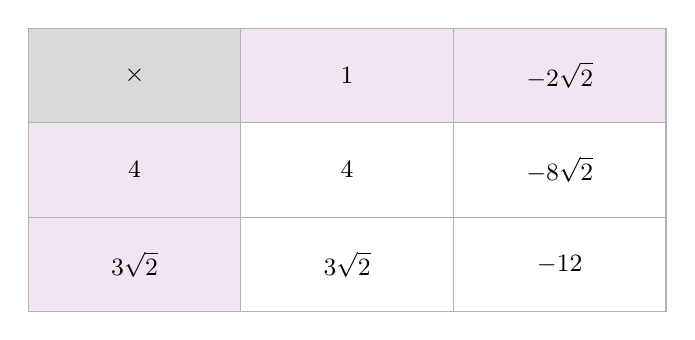
\begin{tikzpicture}[x=1cm,y=1cm,every node/.style={font=\small}]
\fill[gray!30] (0,0) rectangle (2.7,-1.2);
\draw[gray!60] (0,0) rectangle (2.7,-1.2);
\node at (1.35,-0.6) {$\displaystyle \times$};
\fill[violet!10] (2.7,0) rectangle (5.4,-1.2);
\draw[gray!60] (2.7,0) rectangle (5.4,-1.2);
\node at (4.05,-0.6) {$\displaystyle 1$};
\fill[violet!10] (5.4,0) rectangle (8.1,-1.2);
\draw[gray!60] (5.4,0) rectangle (8.1,-1.2);
\node at (6.75,-0.6) {$\displaystyle -2\sqrt{2}$};
\fill[violet!10] (0,-1.2) rectangle (2.7,-2.4);
\draw[gray!60] (0,-1.2) rectangle (2.7,-2.4);
\node at (1.35,-1.8) {$\displaystyle 4$};
\fill[white] (2.7,-1.2) rectangle (5.4,-2.4);
\draw[gray!60] (2.7,-1.2) rectangle (5.4,-2.4);
\node at (4.05,-1.8) {$\displaystyle 4$};
\fill[white] (5.4,-1.2) rectangle (8.1,-2.4);
\draw[gray!60] (5.4,-1.2) rectangle (8.1,-2.4);
\node at (6.75,-1.8) {$\displaystyle -8\sqrt{2}$};
\fill[violet!10] (0,-2.4) rectangle (2.7,-3.6);
\draw[gray!60] (0,-2.4) rectangle (2.7,-3.6);
\node at (1.35,-3) {$\displaystyle 3\sqrt{2}$};
\fill[white] (2.7,-2.4) rectangle (5.4,-3.6);
\draw[gray!60] (2.7,-2.4) rectangle (5.4,-3.6);
\node at (4.05,-3) {$\displaystyle 3\sqrt{2}$};
\fill[white] (5.4,-2.4) rectangle (8.1,-3.6);
\draw[gray!60] (5.4,-2.4) rectangle (8.1,-3.6);
\node at (6.75,-3) {$\displaystyle -12$};
\end{tikzpicture}
}
\end{center}
\small Collect: $4-12=-8$; $-8\sqrt2+3\sqrt2=-5\sqrt2$. Note $3\sqrt2\times(-2\sqrt2)=-6\times2=-12$. Area model (box method): the two binomial terms label the rows and columns; sum the cells, then collect the rational and surd parts.\normalsize

\medskip\hrule

\section*{Laws of Surds 35\quad\small\texttt{(a5-035)}}
\addcontentsline{toc}{section}{Laws of Surds 35 (a5-035)}
\textit{Difficulty: Foundation \quad\textbar\quad Marks: 2}

\question{Expand and simplify: \( (3\sqrt{2} + \sqrt{5})(3\sqrt{2} - \sqrt{5}) \)}

\textbf{Worked solution.}

\textit{Step 1: Apply the difference of two squares: \( (a+b)(a-b) = a^2 - b^2 \).}
\[\begin{gathered}
(3\sqrt{2})^2 - (\sqrt{5})^2
\end{gathered}\]
The brackets are conjugate pairs.

\textit{Step 2: Evaluate each square.}
\[\begin{gathered}
9 \times 2 - 5 = 18 - 5 = 13
\end{gathered}\]
\( (3\sqrt{2})^2 = 9 \times 2 = 18 \) and \( (\sqrt{5})^2 = 5 \).

\begin{answerbox}
\textbf{Final answer:}\quad \(\displaystyle 13\)
\end{answerbox}
\textbf{Diagram.}

\begin{center}
\resizebox{\ifdim\width>\linewidth \linewidth\else \width\fi}{!}{%
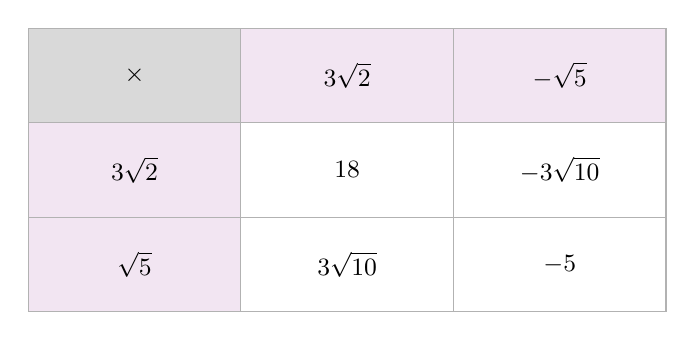
\begin{tikzpicture}[x=1cm,y=1cm,every node/.style={font=\small}]
\fill[gray!30] (0,0) rectangle (2.7,-1.2);
\draw[gray!60] (0,0) rectangle (2.7,-1.2);
\node at (1.35,-0.6) {$\displaystyle \times$};
\fill[violet!10] (2.7,0) rectangle (5.4,-1.2);
\draw[gray!60] (2.7,0) rectangle (5.4,-1.2);
\node at (4.05,-0.6) {$\displaystyle 3\sqrt{2}$};
\fill[violet!10] (5.4,0) rectangle (8.1,-1.2);
\draw[gray!60] (5.4,0) rectangle (8.1,-1.2);
\node at (6.75,-0.6) {$\displaystyle -\sqrt{5}$};
\fill[violet!10] (0,-1.2) rectangle (2.7,-2.4);
\draw[gray!60] (0,-1.2) rectangle (2.7,-2.4);
\node at (1.35,-1.8) {$\displaystyle 3\sqrt{2}$};
\fill[white] (2.7,-1.2) rectangle (5.4,-2.4);
\draw[gray!60] (2.7,-1.2) rectangle (5.4,-2.4);
\node at (4.05,-1.8) {$\displaystyle 18$};
\fill[white] (5.4,-1.2) rectangle (8.1,-2.4);
\draw[gray!60] (5.4,-1.2) rectangle (8.1,-2.4);
\node at (6.75,-1.8) {$\displaystyle -3\sqrt{10}$};
\fill[violet!10] (0,-2.4) rectangle (2.7,-3.6);
\draw[gray!60] (0,-2.4) rectangle (2.7,-3.6);
\node at (1.35,-3) {$\displaystyle \sqrt{5}$};
\fill[white] (2.7,-2.4) rectangle (5.4,-3.6);
\draw[gray!60] (2.7,-2.4) rectangle (5.4,-3.6);
\node at (4.05,-3) {$\displaystyle 3\sqrt{10}$};
\fill[white] (5.4,-2.4) rectangle (8.1,-3.6);
\draw[gray!60] (5.4,-2.4) rectangle (8.1,-3.6);
\node at (6.75,-3) {$\displaystyle -5$};
\end{tikzpicture}
}
\end{center}
\small DOTS: $(3\sqrt2)^2=18$, $(\sqrt5)^2=5$; cross-terms cancel, $18-5=13$. Area model (box method): the two binomial terms label the rows and columns; sum the cells, then collect the rational and surd parts.\normalsize

\medskip\hrule

\section*{Laws of Surds 36\quad\small\texttt{(a5-036)}}
\addcontentsline{toc}{section}{Laws of Surds 36 (a5-036)}
\textit{Difficulty: Foundation \quad\textbar\quad Marks: 1}

\question{Simplify: \( \sqrt{200} \)}

\textbf{Worked solution.}

\textit{Step 1: Find the largest square number that is a factor of 200.}
\[\begin{gathered}
\sqrt{200} = \sqrt{100 \times 2}
\end{gathered}\]
100 is the largest square factor of 200.

\textit{Step 2: Split and simplify.}
\[\begin{gathered}
\sqrt{100} \times \sqrt{2} = 10\sqrt{2}
\end{gathered}\]
\( \sqrt{100} = 10 \).

\begin{answerbox}
\textbf{Final answer:}\quad \(\displaystyle 10\sqrt{2}\)
\end{answerbox}
\textbf{Diagram.}

\begin{center}
\resizebox{\ifdim\width>\linewidth \linewidth\else \width\fi}{!}{%
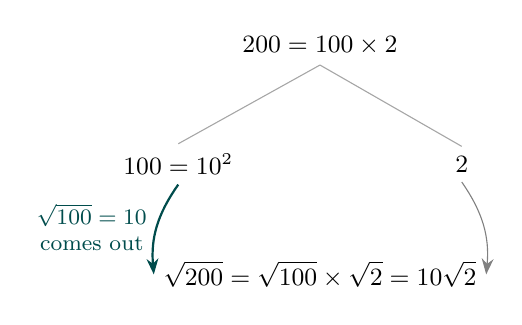
\begin{tikzpicture}[>={Stealth[length=2mm]},every node/.style={font=\small}]
\node (n) at (0,1.5) {$200=100\times 2$};
\node (sq) at (-1.8,0) {$100=10^{2}$};
\node (rem) at (1.8,0) {$2$};
\draw[gray!70] (n.south) -- (sq.north);
\draw[gray!70] (n.south) -- (rem.north);
\node (outc) at (0,-1.4) {$\displaystyle \sqrt{200}=\sqrt{100}\times\sqrt{2}=10\sqrt{2}$};
\draw[->,teal!60!black,thick] (sq.south) to[bend right=20] node[left,font=\footnotesize,align=center]{$\sqrt{100}=10$\\comes out} (outc.west);
\draw[->,gray] (rem.south) to[bend left=20] (outc.east);
\end{tikzpicture}
}
\end{center}
\small Factor tree: split the number into its largest perfect-square factor, then the square root of that factor comes out.\normalsize

\medskip\hrule

\section*{Laws of Surds 37\quad\small\texttt{(a5-037)}}
\addcontentsline{toc}{section}{Laws of Surds 37 (a5-037)}
\textit{Difficulty: Foundation \quad\textbar\quad Marks: 1}

\question{Simplify: \( \sqrt{147} \)}

\textbf{Worked solution.}

\textit{Step 1: Find the largest square number that is a factor of 147.}
\[\begin{gathered}
\sqrt{147} = \sqrt{49 \times 3}
\end{gathered}\]
49 is the largest square factor of 147.

\textit{Step 2: Split and simplify.}
\[\begin{gathered}
\sqrt{49} \times \sqrt{3} = 7\sqrt{3}
\end{gathered}\]
\( \sqrt{49} = 7 \).

\begin{answerbox}
\textbf{Final answer:}\quad \(\displaystyle 7\sqrt{3}\)
\end{answerbox}
\textbf{Diagram.}

\begin{center}
\resizebox{\ifdim\width>\linewidth \linewidth\else \width\fi}{!}{%
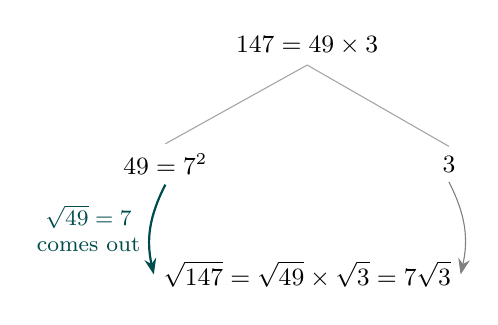
\begin{tikzpicture}[>={Stealth[length=2mm]},every node/.style={font=\small}]
\node (n) at (0,1.5) {$147=49\times 3$};
\node (sq) at (-1.8,0) {$49=7^{2}$};
\node (rem) at (1.8,0) {$3$};
\draw[gray!70] (n.south) -- (sq.north);
\draw[gray!70] (n.south) -- (rem.north);
\node (outc) at (0,-1.4) {$\displaystyle \sqrt{147}=\sqrt{49}\times\sqrt{3}=7\sqrt{3}$};
\draw[->,teal!60!black,thick] (sq.south) to[bend right=20] node[left,font=\footnotesize,align=center]{$\sqrt{49}=7$\\comes out} (outc.west);
\draw[->,gray] (rem.south) to[bend left=20] (outc.east);
\end{tikzpicture}
}
\end{center}
\small Factor tree: split the number into its largest perfect-square factor, then the square root of that factor comes out.\normalsize

\medskip\hrule

\section*{Laws of Surds 38\quad\small\texttt{(a5-038)}}
\addcontentsline{toc}{section}{Laws of Surds 38 (a5-038)}
\textit{Difficulty: Foundation \quad\textbar\quad Marks: 2}

\question{Evaluate: \( 4\sqrt{3} \times 2\sqrt{27} \)}

\textbf{Worked solution.}

\textit{Step 1: Multiply the coefficients and the surds separately.}
\[\begin{gathered}
(4 \times 2) \times (\sqrt{3} \times \sqrt{27}) = 8 \times \sqrt{81}
\end{gathered}\]
\( \sqrt{3} \times \sqrt{27} = \sqrt{3 \times 27} = \sqrt{81} \).

\textit{Step 2: Evaluate.}
\[\begin{gathered}
8 \times 9 = 72
\end{gathered}\]
\( \sqrt{81} = 9 \).

\begin{answerbox}
\textbf{Final answer:}\quad \(\displaystyle 72\)
\end{answerbox}
\textbf{Diagram.}

\begin{center}
\resizebox{\ifdim\width>\linewidth \linewidth\else \width\fi}{!}{%
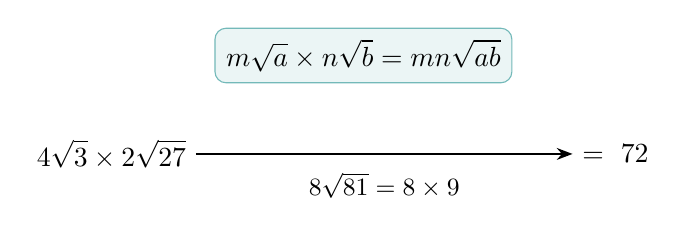
\begin{tikzpicture}[>={Stealth[length=2mm]}]
\node[draw=teal!55,rounded corners,fill=teal!8,inner sep=4pt] (rule) at (3.2,1.25) {$\displaystyle m\sqrt{a}\times n\sqrt{b}=mn\sqrt{ab}$};
\node (L) at (0,0) {$\displaystyle 4\sqrt{3}\times 2\sqrt{27}$};
\node (R) at (6.4,0) {$\displaystyle =\ 72$};
\draw[->,thick] (L) -- (R) node[midway,below=3pt,font=\small,align=center]{$8\sqrt{81}=8\times9$};
\end{tikzpicture}
}
\end{center}
\small Surd-law card: the boxed general rule (teal) is applied to the expression.\normalsize

\medskip\hrule

\section*{Laws of Surds 39\quad\small\texttt{(a5-039)}}
\addcontentsline{toc}{section}{Laws of Surds 39 (a5-039)}
\textit{Difficulty: Foundation \quad\textbar\quad Marks: 3}

\question{Expand and simplify: \( (1 + \sqrt{6})(3 + 2\sqrt{6}) \)}

\textbf{Worked solution.}

\textit{Expand and simplify}
\[\begin{gathered}
\begin{aligned} (1+\sqrt{6})(3+2\sqrt{6}) &= 1(3+2\sqrt{6})+\sqrt{6}(3+2\sqrt{6}) \\ &= 3+2\sqrt{6}+3\sqrt{6}+2(6) \\ &= 3+2\sqrt{6}+3\sqrt{6}+12 \\ &= 15 + 5\sqrt{6} \end{aligned}
\end{gathered}\]
Distribute each term. Note \(\sqrt{6} \times 2\sqrt{6} = 2 \times 6 = 12\). Then collect rational and surd parts.

\begin{answerbox}
\textbf{Final answer:}\quad \(\displaystyle 15 + 5\sqrt{6}\)
\end{answerbox}
\textbf{Diagram.}

\begin{center}
\resizebox{\ifdim\width>\linewidth \linewidth\else \width\fi}{!}{%
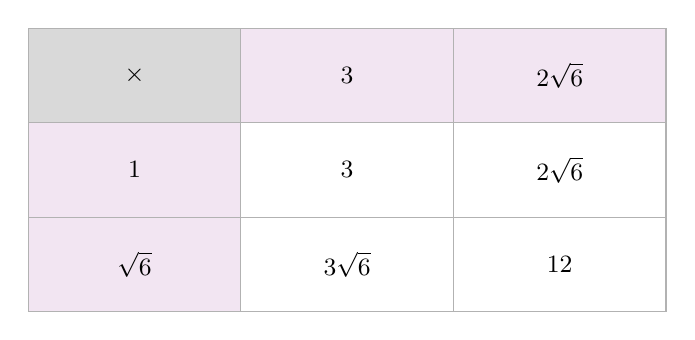
\begin{tikzpicture}[x=1cm,y=1cm,every node/.style={font=\small}]
\fill[gray!30] (0,0) rectangle (2.7,-1.2);
\draw[gray!60] (0,0) rectangle (2.7,-1.2);
\node at (1.35,-0.6) {$\displaystyle \times$};
\fill[violet!10] (2.7,0) rectangle (5.4,-1.2);
\draw[gray!60] (2.7,0) rectangle (5.4,-1.2);
\node at (4.05,-0.6) {$\displaystyle 3$};
\fill[violet!10] (5.4,0) rectangle (8.1,-1.2);
\draw[gray!60] (5.4,0) rectangle (8.1,-1.2);
\node at (6.75,-0.6) {$\displaystyle 2\sqrt{6}$};
\fill[violet!10] (0,-1.2) rectangle (2.7,-2.4);
\draw[gray!60] (0,-1.2) rectangle (2.7,-2.4);
\node at (1.35,-1.8) {$\displaystyle 1$};
\fill[white] (2.7,-1.2) rectangle (5.4,-2.4);
\draw[gray!60] (2.7,-1.2) rectangle (5.4,-2.4);
\node at (4.05,-1.8) {$\displaystyle 3$};
\fill[white] (5.4,-1.2) rectangle (8.1,-2.4);
\draw[gray!60] (5.4,-1.2) rectangle (8.1,-2.4);
\node at (6.75,-1.8) {$\displaystyle 2\sqrt{6}$};
\fill[violet!10] (0,-2.4) rectangle (2.7,-3.6);
\draw[gray!60] (0,-2.4) rectangle (2.7,-3.6);
\node at (1.35,-3) {$\displaystyle \sqrt{6}$};
\fill[white] (2.7,-2.4) rectangle (5.4,-3.6);
\draw[gray!60] (2.7,-2.4) rectangle (5.4,-3.6);
\node at (4.05,-3) {$\displaystyle 3\sqrt{6}$};
\fill[white] (5.4,-2.4) rectangle (8.1,-3.6);
\draw[gray!60] (5.4,-2.4) rectangle (8.1,-3.6);
\node at (6.75,-3) {$\displaystyle 12$};
\end{tikzpicture}
}
\end{center}
\small Collect: $3+12=15$; $2\sqrt6+3\sqrt6=5\sqrt6$. Note $\sqrt6\times2\sqrt6=2\times6=12$. Area model (box method): the two binomial terms label the rows and columns; sum the cells, then collect the rational and surd parts.\normalsize

\medskip\hrule

\section*{Laws of Surds 40\quad\small\texttt{(a5-040)}}
\addcontentsline{toc}{section}{Laws of Surds 40 (a5-040)}
\textit{Difficulty: Foundation \quad\textbar\quad Marks: 3}

\question{Triangle \( PQR \) is right-angled at \( Q \). Side \( PR \) has length \( 7\sqrt{2} \) cm and side \( PQ \) has length \( \sqrt{2} \) cm. Find the length of side \( QR \) in the form \( k\sqrt{6} \) cm, where \( k \) is an integer.}

\textbf{Worked solution.}

\textit{Step 1: Apply Pythagoras's theorem: \(PR^2 = PQ^2 + QR^2\), so \(QR^2 = PR^2 - PQ^2\).}
\[\begin{gathered}
QR^2 = (7\sqrt{2})^2 - (\sqrt{2})^2
\end{gathered}\]
\( PR \) is the hypotenuse (the side opposite the right angle).

\textit{Step 2: Evaluate each square.}
\[\begin{gathered}
QR^2 = 49 \times 2 - 1 \times 2 = 98 - 2 = 96
\end{gathered}\]
\( (7\sqrt{2})^2 = 49 \times 2 = 98 \) and \( (\sqrt{2})^2 = 2 \).

\textit{Step 3: Take the square root and simplify.}
\[\begin{gathered}
QR = \sqrt{96} = \sqrt{16 \times 6} = 4\sqrt{6}
\end{gathered}\]
16 is the largest square factor of 96, and \( \sqrt{16} = 4 \).

\begin{answerbox}
\textbf{Final answer:}\quad \(\displaystyle 4\sqrt{6}\) cm
\end{answerbox}
\textbf{Diagram.}

\begin{center}
\resizebox{\ifdim\width>\linewidth \linewidth\else \width\fi}{!}{%
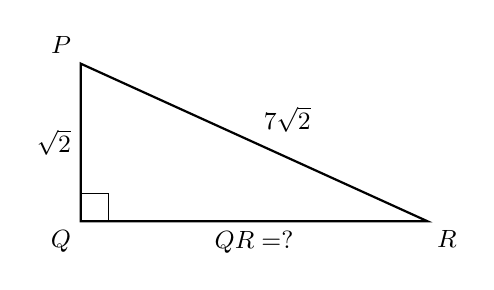
\begin{tikzpicture}[font=\small,>={Stealth[length=2mm]}]
\coordinate (Q) at (0,0);
\coordinate (R) at (4.4,0);
\coordinate (P) at (0,2.0);
\draw[thick] (Q)--(R)--(P)--cycle;
\draw (0.35,0) |- (0,0.35);
\node[below left] at (Q) {$Q$};
\node[below right] at (R) {$R$};
\node[above left] at (P) {$P$};
\node[left] at ($(Q)!0.5!(P)$) {$\sqrt{2}$};
\node[below] at ($(Q)!0.5!(R)$) {$QR=?$};
\node[above right] at ($(P)!0.5!(R)$) {$7\sqrt{2}$};
\end{tikzpicture}
}
\end{center}
\small By Pythagoras, $QR^{2}=PR^{2}-PQ^{2}=(7\sqrt2)^2-(\sqrt2)^2=98-2=96$, so $QR=\sqrt{96}=4\sqrt6$ cm.\normalsize

\medskip\hrule

\end{document}
